\chapter{Solução proposta}\label{chapter:proposed_solution}

O desenvolvimento de uma plataforma colaborativa apresenta diversos desafios ao nível da sua arquitetura, 
do modelo de dados a construir e das decisões de implementação ao longo do seu desenvolvimento. 
\par
Neste capítulo são abordadas as decisões tomadas no desenvolvimento do projeto, tendo em conta a plataforma \textit{OutSystems~\cite{outsystems}}. 
\par
Na secção~\ref{sec:diagram} encontra-se o diagrama de blocos da solução.
\par
Na secção~\ref{sec:arquitechture} encontra-se uma breve análise da arquitetura da plataforma \textit{OutSystems~\cite{outsystems}} e a arquitetura \textit{4 Layer Canvas} desenvolvida.
\par
Na secção~\ref{sec:ModeloDados} encontra-se o modelo de dados e uma síntese do mesmo.
\par 
Na secção~\ref{sec:implementacao} encontram-se todos os detalhes e abordagens adotadas na implementação da solução.

\section{Diagrama de blocos da solução}\label{sec:diagram}
A figura~\ref{fig:diagram} apresenta o diagrama de blocos da plataforma \textit{Corporate Collaboration}. 
\par
No mesmo constam as permissões (\textit{roles}) que um utilizador registado pode apresentar e quais as funcionalidades a que cada \textit{role} pode aceder nos módulos constituintes da aplicação, \textit{UserEndPoints} e \textit{Back-Office}. 

\begin{figure}[H]
  \centering
  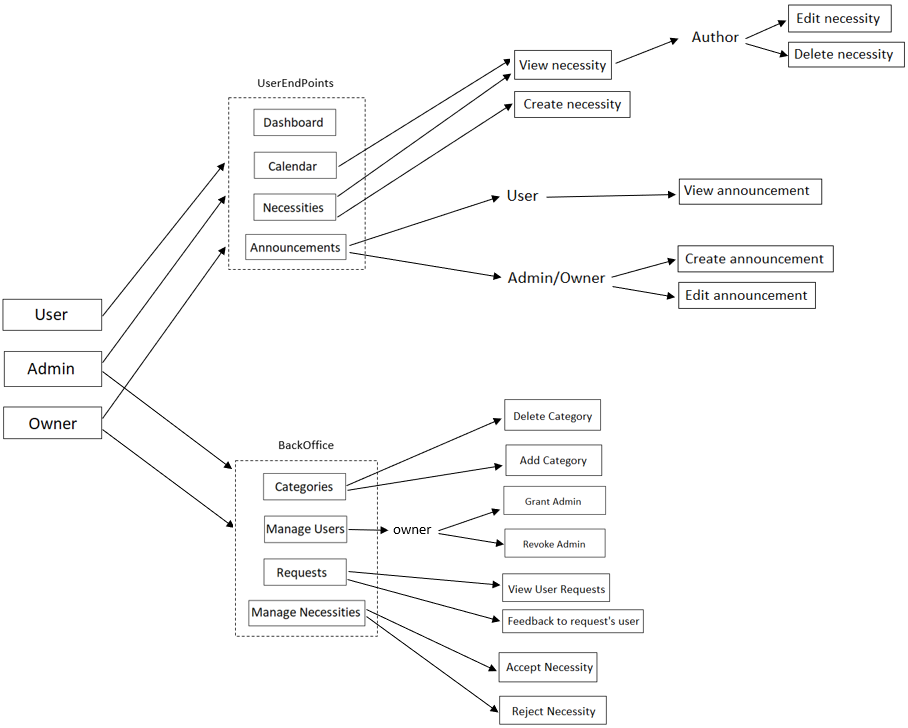
\includegraphics[scale=0.5]{figures/Diagrama de blocos.png}
  \caption{Diagrama de blocos da aplicação}\label{fig:diagram}
\end{figure}

\newpage

\section{Arquitetura}\label{sec:arquitechture}

\subsection{Plataforma \textit{OutSystems}}\label{sec:OutSystemsArch}

A arquitetura desta plataforma pode ser observada na figura~\ref{fig:outsystemsArch}. 
O principal componente da plataforma é o Platform Server~\cite{outsystemsPlatformServer} que permite que as aplicações 
desenvolvidas sejam geradas, optimizadas, compiladas e publicadas. 

\begin{figure}[H]
  \centering
  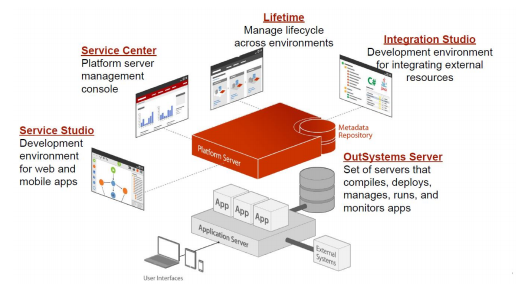
\includegraphics[]{figures/Architecture.png}
  \caption{Arquitetura da plataforma \textit{OutSystems~\cite{outsystems}}}\label{fig:outsystemsArch}
\end{figure}

Este componente usa os seguintes serviços: 
\begin{enumerate}
  \item \textit{Code Generator} --- Usa a aplicação modelada no \textit{Service Studio} e gera o código necessário usando tecnologias standard (como \textit{.NET, SQL Server, HTML,} etc.) para a criação de uma aplicação optimizada e segura.
  \item \textit{Deployment Services} --- Publica o código que foi previamente gerado no servidor, assegurando que a aplicação é instalada consistentemente em cada front-end da infraestrutura.
  \item \textit{Application Services} --- Gere as aplicações durante o runtime, através da execução de \textit{batches} agendados e serviços de \textit{logging} assíncronos que permitem que sejam armazenados eventos como erros, inspeções e métricas de desempenho.
\end{enumerate}

\newpage

\subsection{Arquitetura 4 Layer Canvas}\label{sec:4lc}

Para desenharmos a arquitetura da nossa solução, seguimos a metodologia da plataforma \textit{OutSystems~\cite{outsystems}}, a \textit{4 Layer Canvas} apresentado na figura~\ref{fig:4lc}.

\begin{figure}[H]
  \centering 
  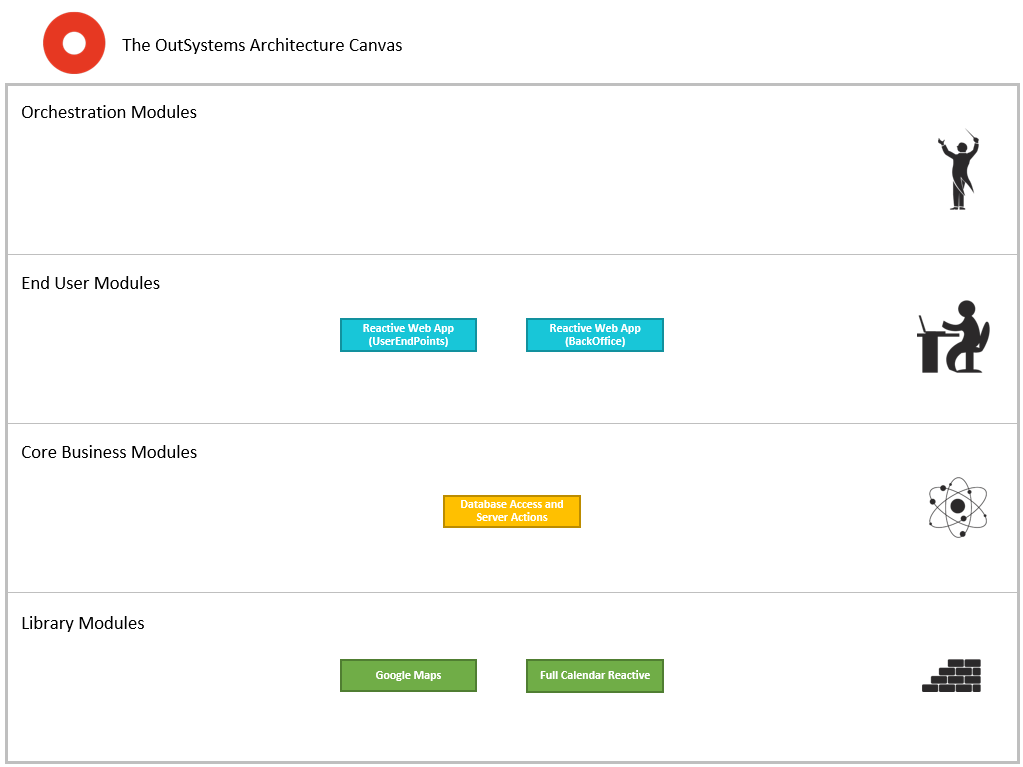
\includegraphics[scale=0.5]{figures/4LayerCanvas.png}
  \caption{4 \textit{Layer Canvas}}\label{fig:4lc}
\end{figure}

Esta metodologia propõe que se estruture as várias funcionalidades da aplicação por quatro camadas, sendo estas, começando por baixo: 

\begin{itemize}
    \item \textit{Library Layer} --- Aqui devem constar os módulos que são transversais ao domínio do problema, tais como: temas, bibliotecas, etc. 
    \item \textit{Core Layer} --- Módulos referentes à lógica de negócio, modelo de dados e \textit{server actions}. 
    \item \textit{End User Layer} --- Nesta camada é tratada toda a parte de interface e experiência do utilizador, fazendo uso das camadas anteriores. 
    \item \textit{Orchestration Layer} --- Camada que coordena a comunicação entre várias aplicações. 
\end{itemize}

É importante verificar que, apesar da metodologia apresentar quatro camadas, 
a nossa arquitetura apenas faz uso das primeiras três devido ao facto do projeto consistir em apenas uma aplicação reactive, 
e não havendo necessidade de coordenar interações com outras aplicações na camada de orquestração. 
Posto isto, a nossa aplicação assenta sobre cinco módulos, representados pela figura~\ref{fig:4lc}.

Começando pela \textit{Library Layer} verificamos que são utilizados os módulos relativos à integração da aplicação 
com o \textit{Google Maps}, o que possibilita a apresentação de mapas nos recursos de uma necessidade (descrito na subsecção~\ref{subsec:implementacao:necessityCreation}), e com o \textit{Full Calendar Reactive} que é utilizado para apresentar o calendário no ecrã \textit{Calendar} descrito na subsecção~\ref{subsec:implementacao:calendarNecessitiesView}. 

\par
De seguida temos a \textit{ Core Layer}, 
onde definimos as entidades de domínio e operações de acesso ao servidor. Toda esta dinâmica está implementada através do módulo \textit{ServerLogic}, onde é coordenada toda a lógica de negócio da aplicação. 
\par
Por fim a \textit{ End User Layer} onde são definidos os módulos \textit{UserEndPoints} e \textit{Back-Office} que suportam os ecrãs e a lógica de cliente. 
\par
O tema apresentado em ambos os módulos foi desenvolvido pelo grupo, devido ao facto da solução ser concretizada como uma aplicação \textit{web reactive} e não haver temas já implementados na \textit{forge} da \textit{OutSystems} para este tipo de aplicação. 
O mesmo foi desenvolvido através da manipulação de \textit{CSS} e de ajustamentos cuidados para apresentar uma \textit{User Interface} apelativa.

\newpage

\section{Modelo de Dados}\label{sec:ModeloDados}

O modelo Entidade-Associação da solução desenvolvida pode ser consultado no anexo~\ref{anexo:modeloEA}
O conceito predominante no modelo de dados, (figura~\ref{fig:modeloDados}), é o de necessidade, representado pela tabela \textit{Necessity}.

\begin{figure}[H]
  \centering 
  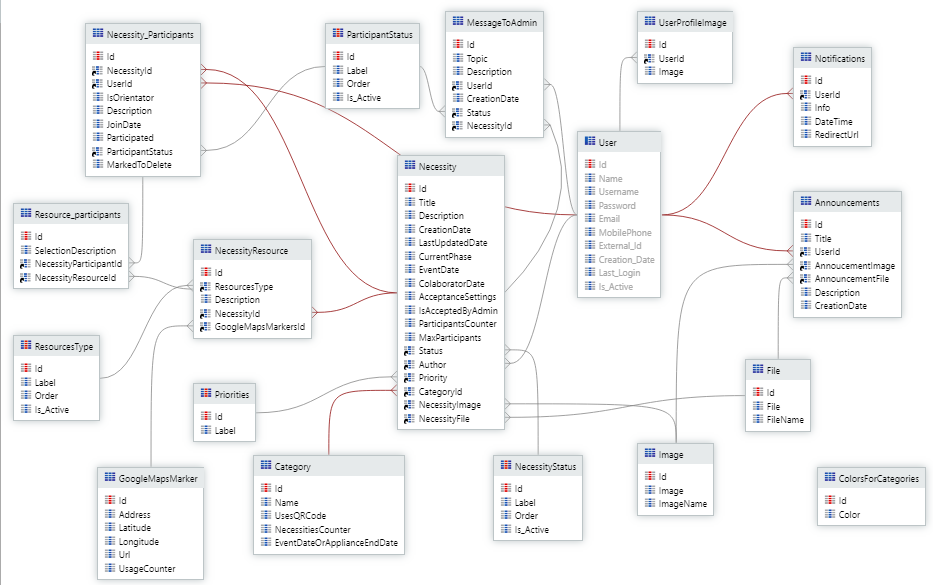
\includegraphics[scale=0.5]{figures/DataModel.png}
  \caption{Modelo de dados}\label{fig:modeloDados}
\end{figure}

 
Uma necessidade é caracterizada por diversos elementos dos quais destacamos o \textit{Status} que referencia uma tabela estática (\textit{NecessityStatus}) que contém os valores possíveis do estado da necessidade, 
podendo ter os valores \textit{\" Closed\"}, \textit{\" Active\" } ou \textit{\" Archived \".} 
\par
A \textit{CurrentPhase} que indica a fase de candidaturas atual, 
podendo ser para colaboradores ou participantes, a \textit{ColaboratorDate} que representa a data limite das candidaturas 
à posição de colaborador, \textit{AcceptanceSettings} que indica se para a necessidade em causa são aceites todos os participantes ou se existe uma filtragem por parte do autor, 
\textit{isAcceptedByAdmin} que indica se a necessidade criada já foi aceite por um administrador ou pelo \textit{owner} no \textit{back-office}, 
\textit{ParticipantsCounter} que indica o número de participantes desta necessidade, e por último, \textit{MaxParticipants} que serve para guardar o número máximo de participantes que podem existir nesta necessidade. 
\par
As tabelas \textit{NecessityImage} e \textit{NecessityFile} existem para o propósito de guardar ficheiros, 
aliviando a quantidade de dados guardada em cada tuplo \textit{Necessity}, 
seguindo também as boas práticas da plataforma \textit{OutSystems~\cite{outsystems}}.
\par
A entidade estática \textit{Priorities} contém os valores possíveis das prioridades que cada necessidade pode ter.
\par
Associado ao conceito de necessidade está o de recurso, que tem como objetivo acrescentar informação à necessidade de uma forma flexível. 
Para suportar este conceito foi definida a entidade estática \textit{ResourcesType} cujos valores representam os tipos de recursos que um utilizador pode, facultativamente, acrescentar à necessidade, consistindo em acomodação, restaurante e menus de refeições, localização do evento ou transporte. 
A representação de um recurso no modelo de dados traduz-se na entidade \textit{NecessityResource} que guarda informações de cada recurso como o seu tipo (referência à tabela  \textit{ResourcesType}), a sua descrição, o id da necessidade a que o mesmo pertence e, como todos os recursos à exceção do relativo ao transporte têm um mapa do \textit{Google Maps} associado
, o último atributo da tabela \textit{NecessityResource} é um id do marcador do mapa associado ao recurso.
\par
Com o objetivo de guardar informação sobre os participantes de uma necessidade, é definida a entidade \texttt{\textit{Necessity\char`_Participants}} que 
contempla o identificador da necessidade, o identificador do utilizador, a descrição associada à candidatura, 
se esta candidatura é para posição de colaborador ou de participante, a data da candidatura, se o utilizador participou na necessidade, qual o estado da candidatura (dado pela entidade estática \textit{ParticipantStatus}, cujos valores representam se a candidatura está pendente - \textit{pending}, aceite - \textit{accepted} ou rejeitada - \textit{rejected}) e se este participante pediu para remover a sua participação na necessidade e está assinalado para remoção da lista de participantes. 
\par
De modo a que seja possível guardar informação sobre se um participante vai usufruir dos recursos associados a uma necessidade, é definida a entidade \texttt{\textit{Resource\char`_Participants}}.
Esta entidade guarda informações como a descrição da escolha do recurso, o id do participante e o id do recurso.
\par
Com o intuito de suportar a funcionalidade de envio de mensagens entre utilizadores comuns e utilizadores com permissões mais elevadas, foi criada a tabela \textit{MessageToAdmin}. 
Esta tabela tem os atributos necessários para armazenar o tópico de uma mensagem, o seu conteúdo, o utilizador que a criou, a sua data de criação e, por último, o estado da mesma, que pode tomar os valores presentes na entidade estática \textit{ParticipantStatus}. 
Estes valores são \textit{accepted} para mensagens cujo conteúdo foi cumprido ou aceitado, \textit{rejected} para mensagens cujo conteúdo não o foi e \textit{pending} para aquelas que ainda não obtiveram resposta.
\par
Os comunicados feitos na plataforma são suportados pela entidade \textit{Announcements}. 
\par
As notificações apresentadas na plataforma são suportadas pela entidade \textit{Notifications} em que cada notificação está associada a um utilizador através do seu id, o seu conteúdo é guardado no atributo \textit{Info} e a hora da emissão da notificação no atributo \textit{DateTime}. 
\par
Um utilizador que tenha a permissão de administrador, cujos privilégios incluem editar as categorias representadas pela entidade \textit{Category}. Esta entidade tem como atributos o nome da categoria criada, se é uma categoria cujas necessidades vão necessitar de confirmação de presença através de \textit{QR Code}, quantidade de necessidades criadas associadas a esta categoria e se o dia do evento presente em cada necessidade associada a esta categoria corresponde ao dia em que o evento tem lugar ou simplesmente ao final da data de candidaturas. 
\par
Um pequeno exemplo para melhor entendimento deste último atributo é, numa categoria que tenha como conceito a procura de utilizadores para desenvolver peças de software a data associada ás necessidades (atributo \textit{eventDate} da entidade \textit{Necessity}) é de fim da fase de candidaturas para produzir a peça de software em questão, enquanto que uma categoria que tenha como conceito atividades lúdicas terá o atributo \textit{eventDate} das suas necessidades como a data em que o evento irá ocorrer.

\newpage

\section{Implementação}\label{sec:implementacao}

\subsection{Autenticação}\label{subsec:implementacao:login}

Para realizar a autenticação de um utilizador, este introduz as suas credenciais nos respetivos \textit{input fields} e clica no botão \textit{Login}.
Se as credenciais introduzidas não corresponderem às de nenhum utilizador na base de dados, será apresentada uma mensagem de erro.
\par
Um utilizador só terá acesso a outros ecrãs se tiver autenticado, caso contrário será redirecionado para este ecrã, figura~\ref{fig:LoginScreen}.

\begin{figure}[H]
  \centering 
  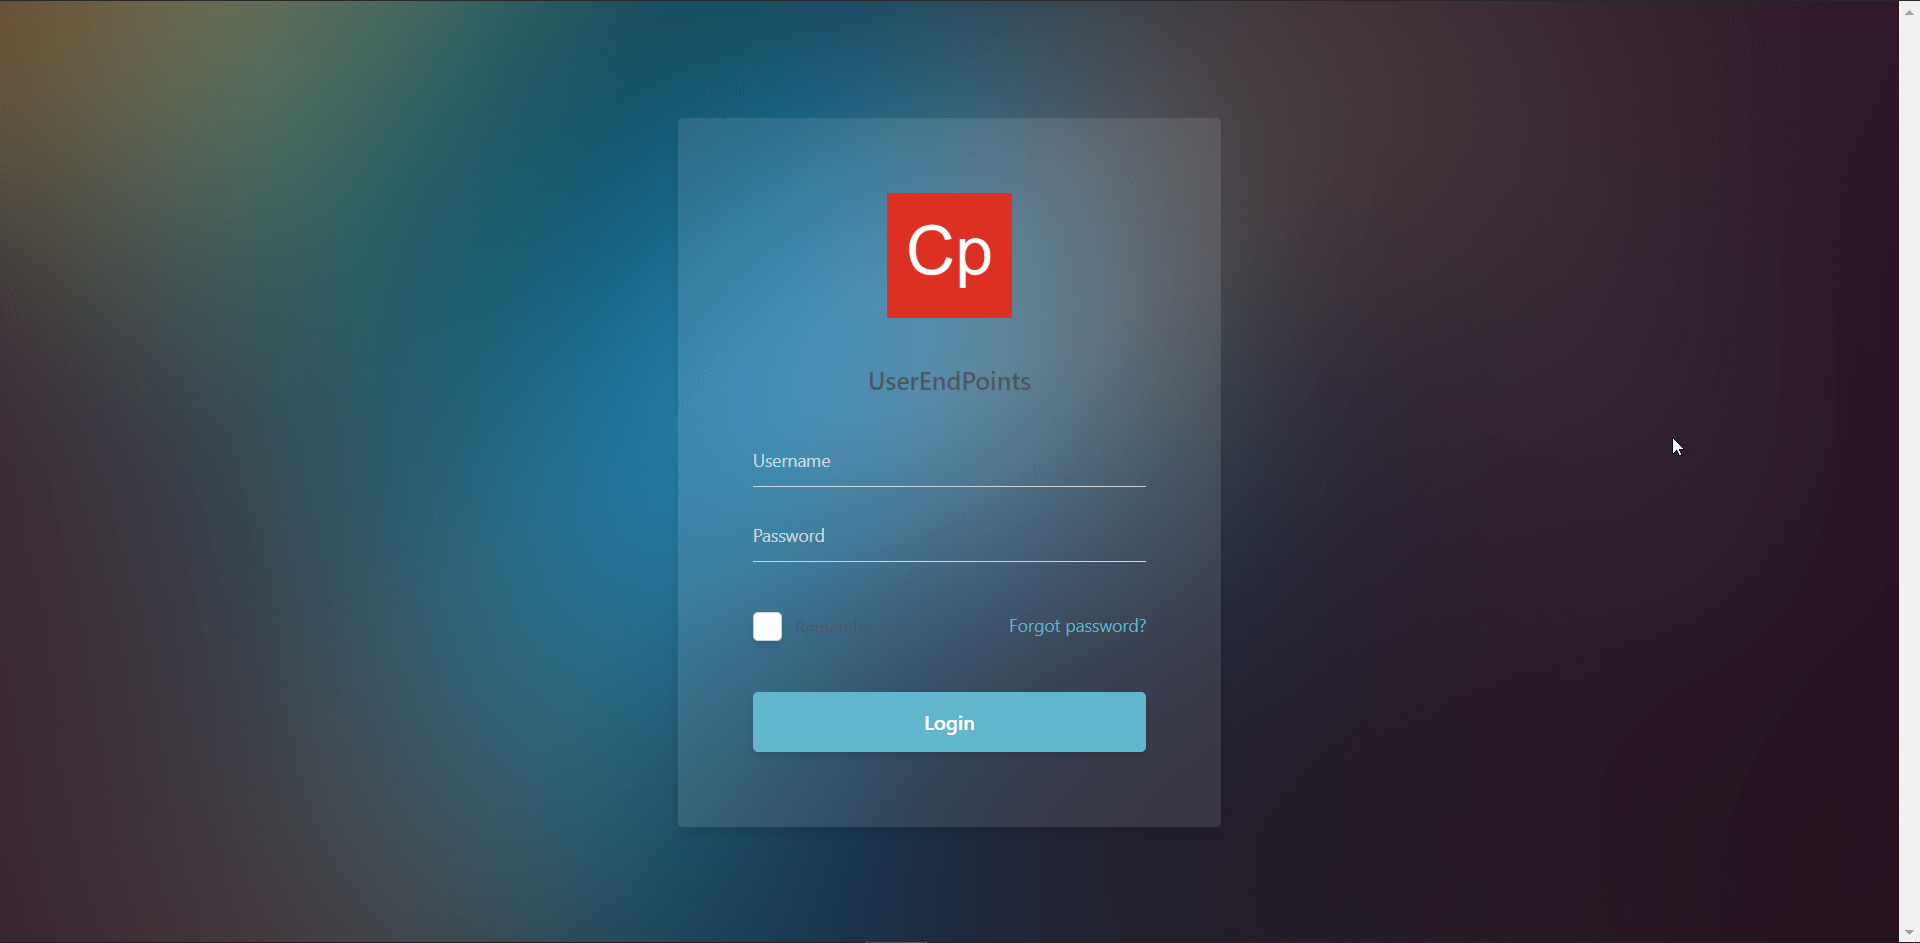
\includegraphics[scale=0.35]{figures/LoginScreen.png}
  \caption{Ecrã de autenticação}\label{fig:LoginScreen}
\end{figure}

\newpage

\subsection{\textit{Back-office}}\label{subsec:implementacao:back-office}

O \textit{back-office} da \textit{Collaboration Platform} tem como principal motivação a manutenção da mesma e o acesso a funcionalidades que requerem permissões superiores, nomeadamente de \textit{admin} ou de \textit{owner}.
Posto isto, o \textit{back-office} é implementado num novo módulo e apresenta quatro ecrãs distintos. 
\par
No ecrã \textit{Necessities} os utilizadores com acesso ao \textit{back-office} têm a possibilidade de verificar as necessidades criadas pela comunidade da empresa, podendo aceitá-las ou eliminá-las. 
Estas necessidades são apresentadas sobre a forma de uma lista, tal como demonstrado na figura~\ref{fig:backoffice_necessities}. Ao pressionar uma delas, serão apresentados os detalhes da mesma e dois ícones que permitirão aceitar ou rejeitar. 

\begin{figure}[H]
  \centering 
  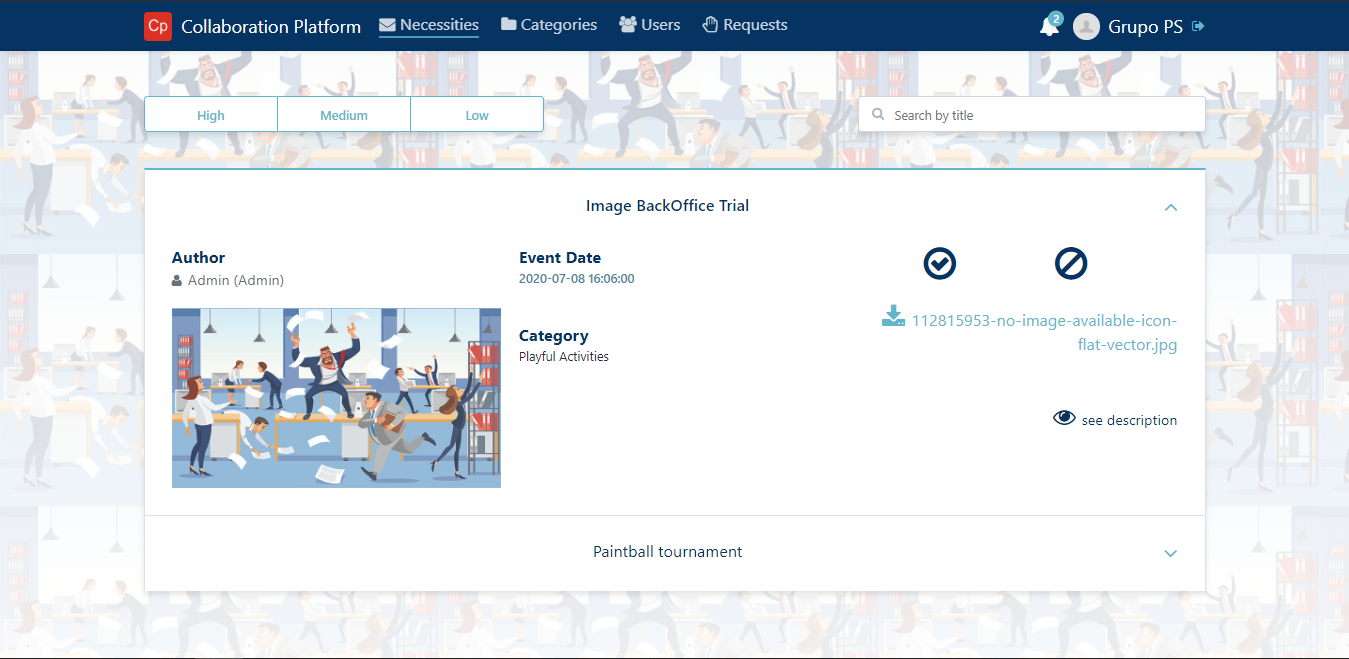
\includegraphics[scale=0.35]{figures/backoffice_necessities.png}
  \caption{Ecrã das necessidades no back-office}\label{fig:backoffice_necessities}
\end{figure}



O ecrã \textit{Categories} tem como objetivo a criação e remoção de categorias. 
As mesmas são apresentadas numa tabela, como é possível verificar na figura figura~\ref{fig:backoffice_categories}, e cada uma tem uma checkbox associada que, quando selecionada, irá deixar a categoria apta para ser eliminada, ao carregar no botão delete. 
Para criar uma nova, basta carregar no botão create e preencher o nome, se é necessária verificação de presenças por \textit{QR Code} e como é interpretada a data de evento de uma necessidade associada a esta nova categoria.

\begin{figure}[H]
  \centering 
  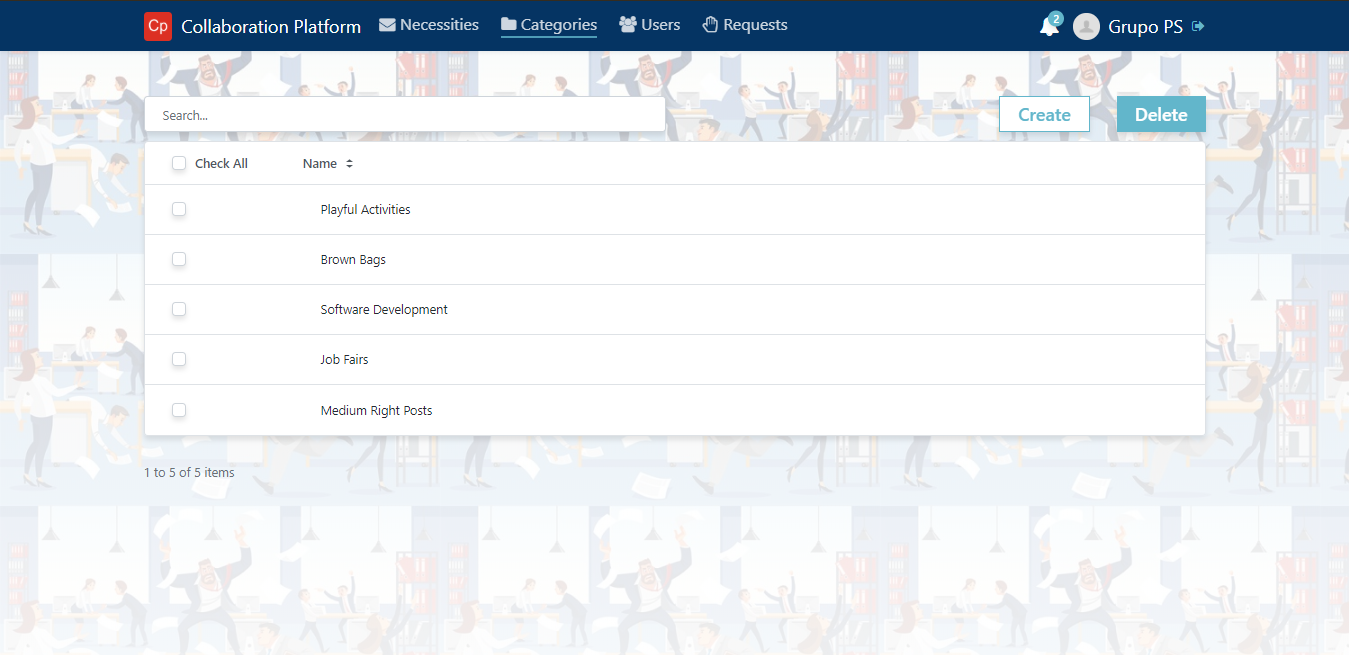
\includegraphics[scale=0.35]{figures/backoffice_categories.png}
  \caption{Ecrã das categorias}\label{fig:backoffice_categories}
\end{figure}

\newpage

No ecrã \textit{ManageUsers} é possível ver todos os utilizadores da plataforma separados entre utilizadores comuns e utilizadores com permissões mais elevadas, através de duas \textit{tabs}.
Deste modo, na tab dos utilizadores comuns (representada na figura figura~\ref{fig:backoffice_users_users}) existe a possibilidade de alterar as permissões associadas a um utilizador, concedendo-lhe permissões superiores através do botão \textit{Grant admin}.
Na tab de \textit{Admins}, apresentada na figura figura~\ref{fig:backoffice_users_admin}, existe a possibilidade de despromover um utilizador de administrador a utilizador comum, através do botão \textit{revoke admin}. 
\par
Estas mudanças de \textit{roles} apenas podem ser feitas pelo \textit{owner}, a entidade superior da hierarquia de \textit{roles}. Um utilizador com permissões de administrador apenas pode ver os utilizadores e o seu \textit{role}. 

\begin{figure}[H]
  \centering 
  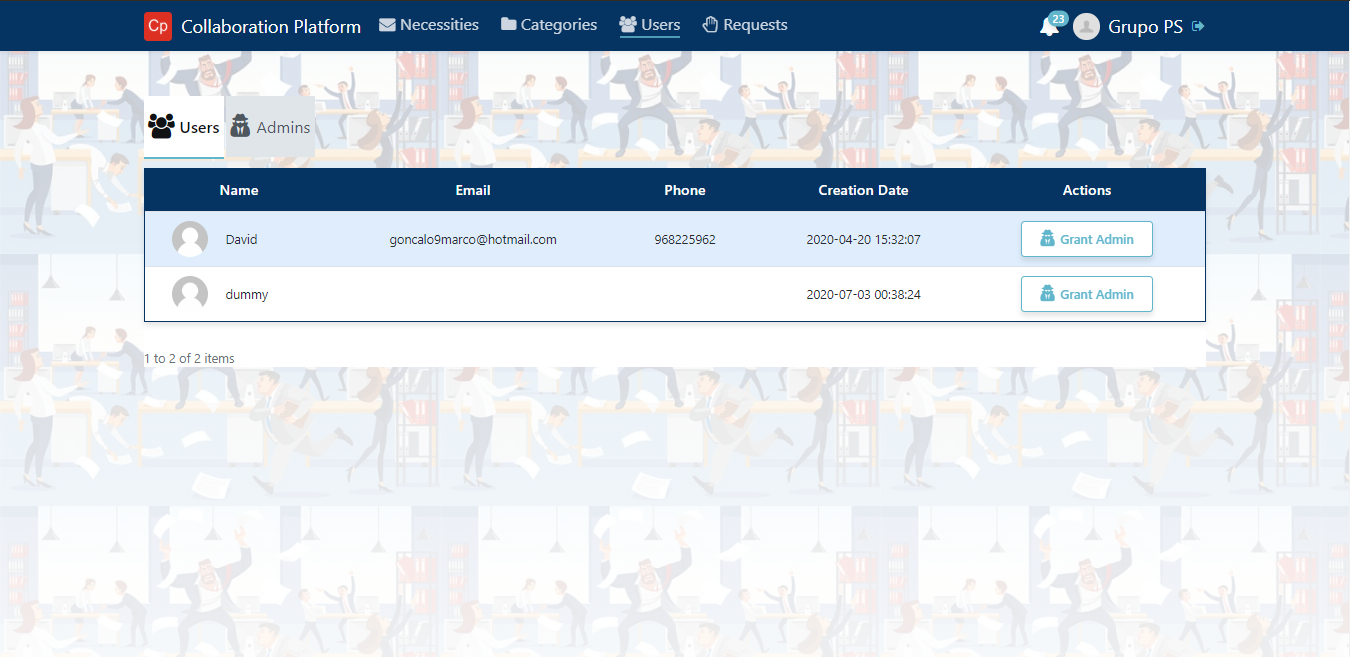
\includegraphics[scale=0.35]{figures/backoffice_users_users.png}
  \caption{Ecrã \textit{ManageUsers} com a tab dos utilizadores comuns ativa }\label{fig:backoffice_users_users}
\end{figure}



\begin{figure}[H]
  \centering 
  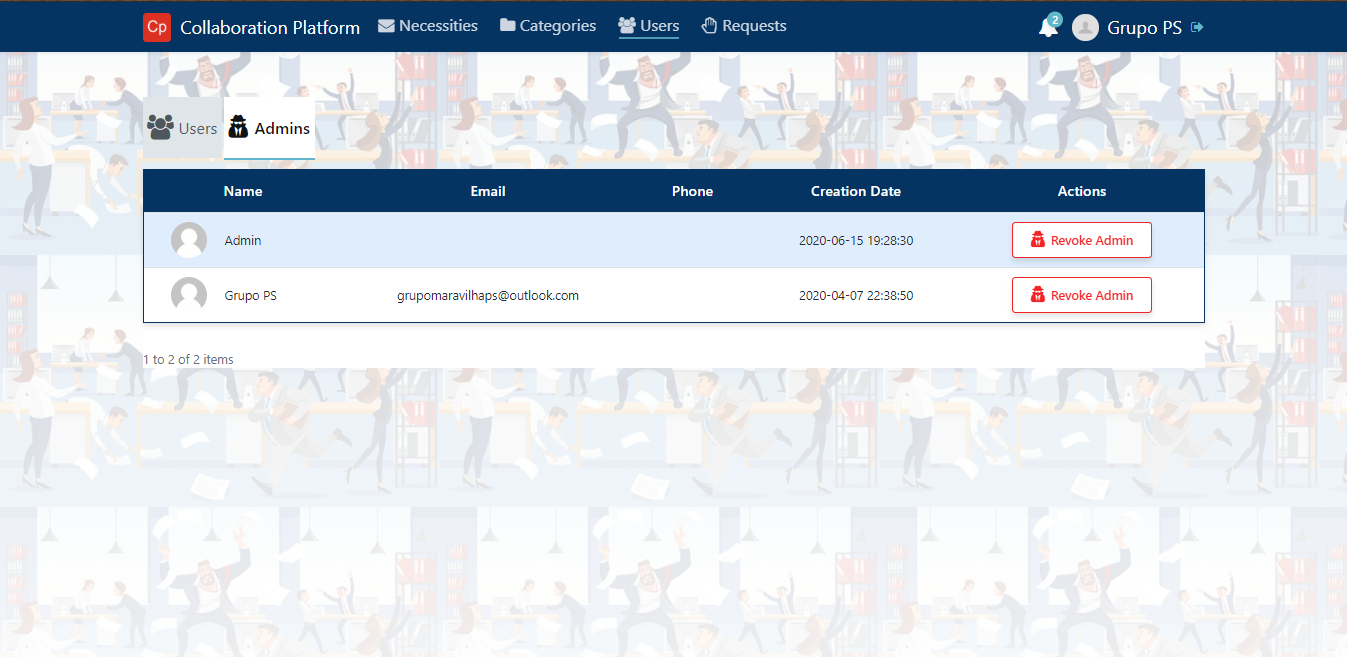
\includegraphics[scale=0.35]{figures/backoffice_users_admin.png}
  \caption{Ecrã \textit{ManageUsers} com a tab dos \textit{admins} e \textit{owner} ativa }\label{fig:backoffice_users_admin}
\end{figure}

Com o intuito de ver as mensagens criadas pela comunidade da empresa, o ecrã \textit{UserMessages} (figura~\ref{fig:backoffice_user_messages}) apresenta-as sobre a forma de uma lista e,
ao carregar numa mensagem, é apresentado o detalhe da mesma. 
\par
Cada utilizador com permisssões para aceder ao \textit{back-office} pode sinalizar uma mensagem que esteja por resolver (\textit{"unresolved"}) como  resolvida (\textit{"resolved"}) se aceitar/cumprir o conteúdo da mensagem ou como \textit{"rejected"} se não for o caso.  

\begin{figure}[H]
  \centering 
  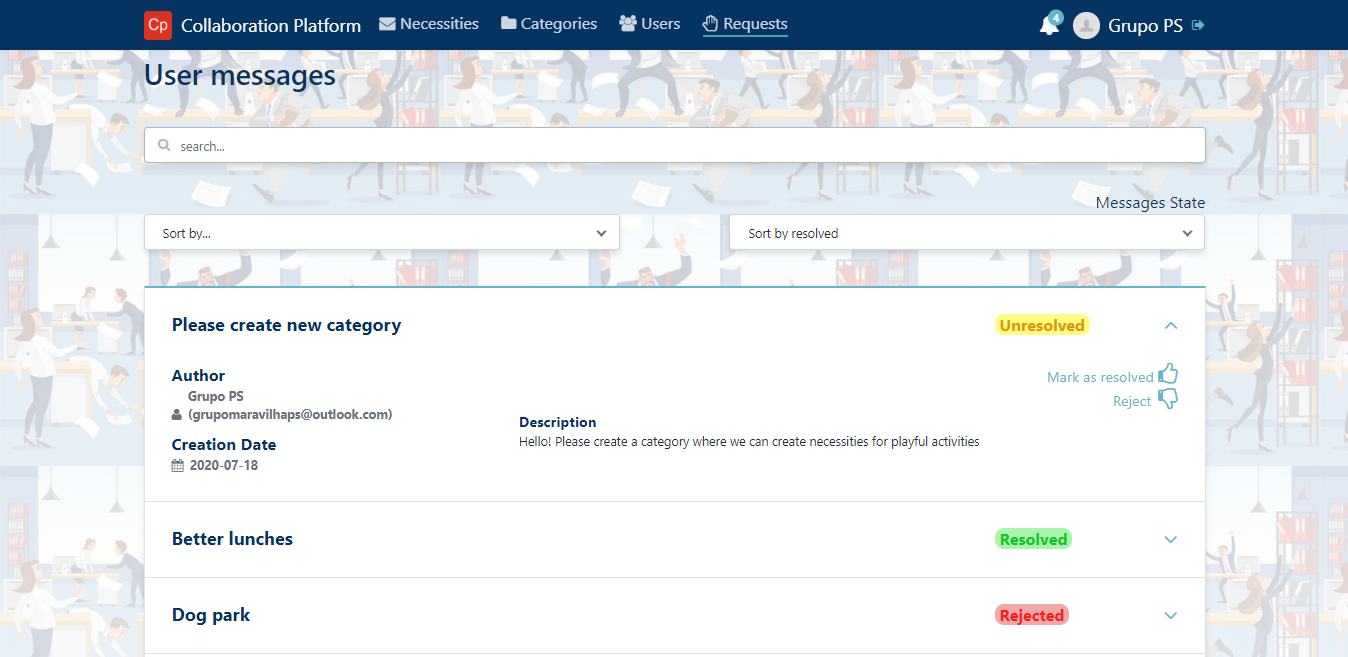
\includegraphics[scale=0.35]{figures/backoffice_userMessages.png}
  \caption{Ecrã \textit{UserMessages}}\label{fig:backoffice_user_messages}
\end{figure}

\newpage

\subsection{\textit{Dashboard}}\label{subsec:implementacao:dashboard}

A um utilizador autenticado é apresentado o ecrã \textit{dashboard}, apresentado na figura~\ref{fig:Dashboard}, assim que inicia sesssão na aplicação.
\par
O mesmo apresenta quatro \textit{widgets} que apresentam informação sobre o número de utilizadores que estão \textit{logged in} e o número de necessidades abertas com as suas respetivas prioridades (\textit{high, medium, low}).
\par
Este ecrã apresenta também um \textit{widget carousel}, com a descrição \textit{"Recently created necessities"}, a partir do qual é possível observar as necessidades que foram criadas mais recentemente. 
\par
Posto isto, do lado direito do \textit{widget carousel}, é demonstrado ao utilizador um gráfico com informação sobre as cinco categorias existentes que apresentam um maior número de necessidades criadas.
A seleção de uma categoria do gráfico promove a navegação para o ecrã das necessidades,  apresentando a lista das mesmas que pertencem à categoria selecionada.
\par
Para cada uma das prioridades que as necessidades podem ter, é apresentado um \textit{ranking} dos utilizadores que mais criaram necessidades, com a respetiva prioridade.

\begin{figure}[H]
  \centering 
  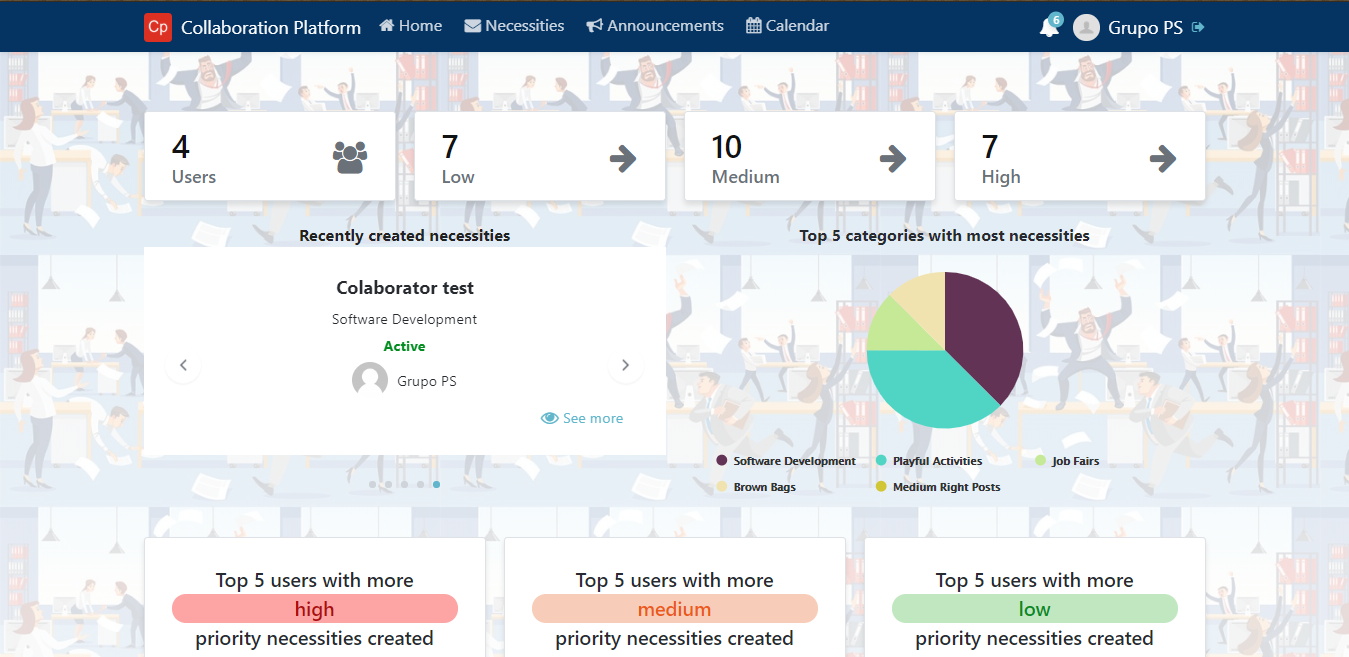
\includegraphics[scale=0.4]{figures/Dashboard.png}
  \caption{\textit{Dashboard}}\label{fig:Dashboard}
\end{figure}

\newpage

\subsection{Visualização de necessidades}\label{subsec:implementacao:necessities}
O utilizador ao carregar no botão \textit{Necessities} presente na barra da aplicação, será redirecionado para o ecrã responsável pela apresentação das necessidades, demonstrado na figura~\ref{fig:NecessitiesScreen}. 
\par
O intuito do mesmo consiste na apresentação das necessidades criadas pela comunidade empresarial, sendo possível aplicar filtros e/ou pesquisar pelo título de uma necessidade de modo a que sejam apresentadas apenas as necessidades alvo.
\par
As necessidades são apresentadas num \textit{widget} tabela, cujas colunas apresentam informação relevante como título, categoria, prioridade, estado, data de criação, data em que a necessidade irá decorrer e o número de participantes. 
\par
Sempre que o utilizador pretender criar uma nova necessidade, apenas tem que carregar no botão \textit{Create Necessity} e será redirecionado para um novo ecrã, onde poderá completar a criação.
\par
A seleção do título de uma necessidade promove a navegação para o ecrã dos detalhes da mesma.
\par
A barra de pesquisa permite que o utilizador procure uma necessidade pelo seu título.
Os filtros aplicáveis são apresentados em dois \textit{dropdowns}, um para permitir a escolha de qual a prioridade e outro para seleção da(s) categoria(s).
\par
O \textit{ widget switch} presente neste ecrã com a descrição \textit{"show only my necessities"}, quando ativo, reorganiza a tabela das necessidades de modo a só mostrar as que o utilizador é autor.
\par
É importante referir que todas as necessidades apresentadas neste ecrã foram previamente aceites por um utilizador com \textit{role} de \textit{admin} ou \textit{owner} no \textit{back-office}, com exceção de quando o \textit{switch} de mostrar apenas as necessidades do utilizador está ativo. 
Neste caso, as necessidades aparecem mesmo que ainda não tenham sido aceites, mas apenas ao utilizador que neste caso é sempre o autor das mesmas. 
\par
Sempre que exista uma mudança na seleção de algum dos \textit{widgets} de filtragem de necessidades ou uma introdução de texto na barra de pesquisa, a tabela é atualizada para apresentar apenas aquelas que verifiquem as características alvo. 
\par
As informações de cada uma das necessidades, das categorias existentes e das prioridades são obtidas comunicando com o servidor através de \textit{Aggregates}. 
\par
Os \textit{Aggregates} são \textit{querys} optimizadas à base de dados de modo a retornar informação de forma eficiente e apresentá-la nos \textit{widgets} do ecrã.

\begin{figure}[H]
  \centering 
  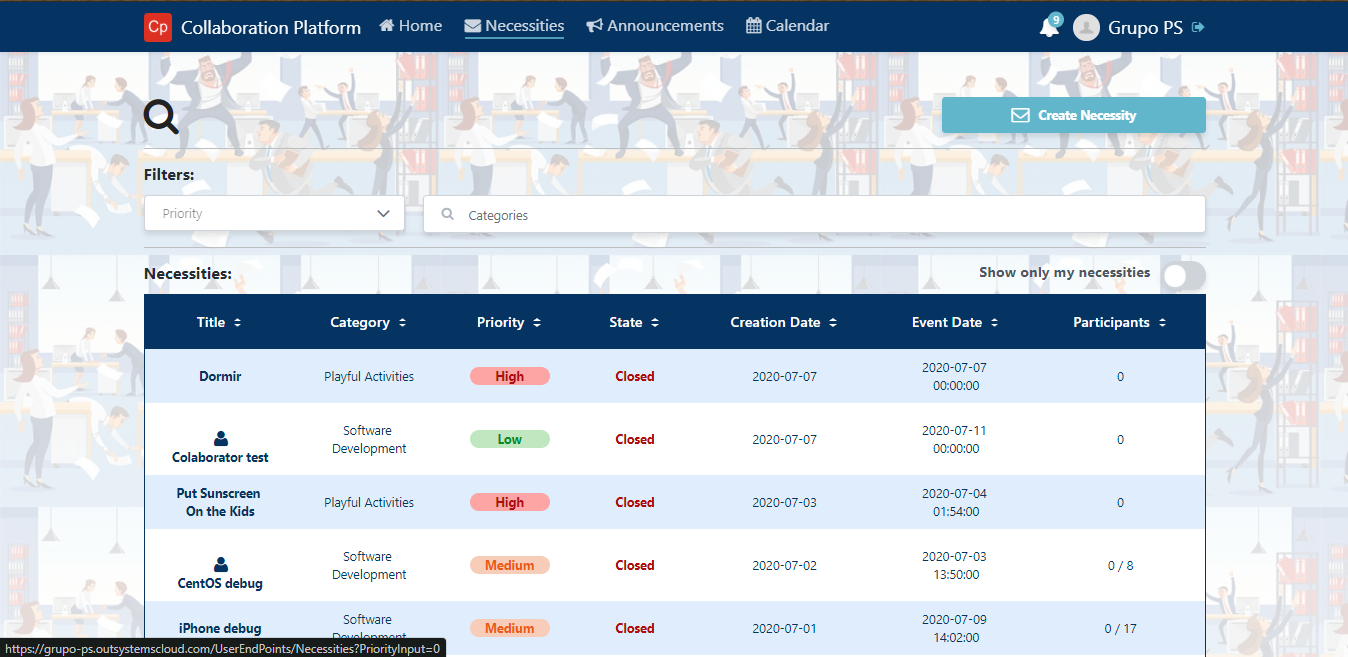
\includegraphics[scale=0.3]{figures/NecessitiesGeneralScreen.png}
  \caption{Ecrã das necessidades.}\label{fig:NecessitiesScreen}
\end{figure}

\newpage

\subsection{Visualização de necessidades num calendário}\label{subsec:implementacao:calendarNecessitiesView}

O utilizador ao carregar no botão \textit{Calendar} presente na barra da aplicação, será redirecionado para o ecrã (figura~\ref{fig:CalendarScreen}) responsável por mostrar, num calendário, todas as necessidades existentes organizadas por datas. 
\par
O objetivo deste ecrã é apresentar de uma forma mais organizada e estruturada todas as necessidades criadas pela empresa, sendo possível filtrá-las. 
\par
Foi utilizado o componente \textit{FullCalendarReactive}, presente na \textit{forge} da plataforma \textit{OutSystems}, de modo a apresentar ao utilizador um calendário interativo.
Para preencher o calendário, para cada necessidade, é criado um objeto \textit{Event} com a sua informação. 
\par
Cada necessidade estará representada no calendário com uma cor diferente de forma a distinguir entre necessidades criadas pelo utilizador, necessidades associadas, nomeadamente em que o utilizador participa, e necessidades criadas por outros utlizadores.
Se o utilizador carregar numa necessidade, este é redirecionado para o seu ecrã de detalhe. 
\par
É possível filtrar necessidades pela sua categoria, através de um \textit{popover menu} que contém todas as categorias existentes. 
Caso seja selecionada uma categoria, são removidas todas as necessidades presentes no calendário, e de seguida, o mesmo é renderizado com as novas necessidades filtradas.

\begin{figure}[H]
  \centering 
  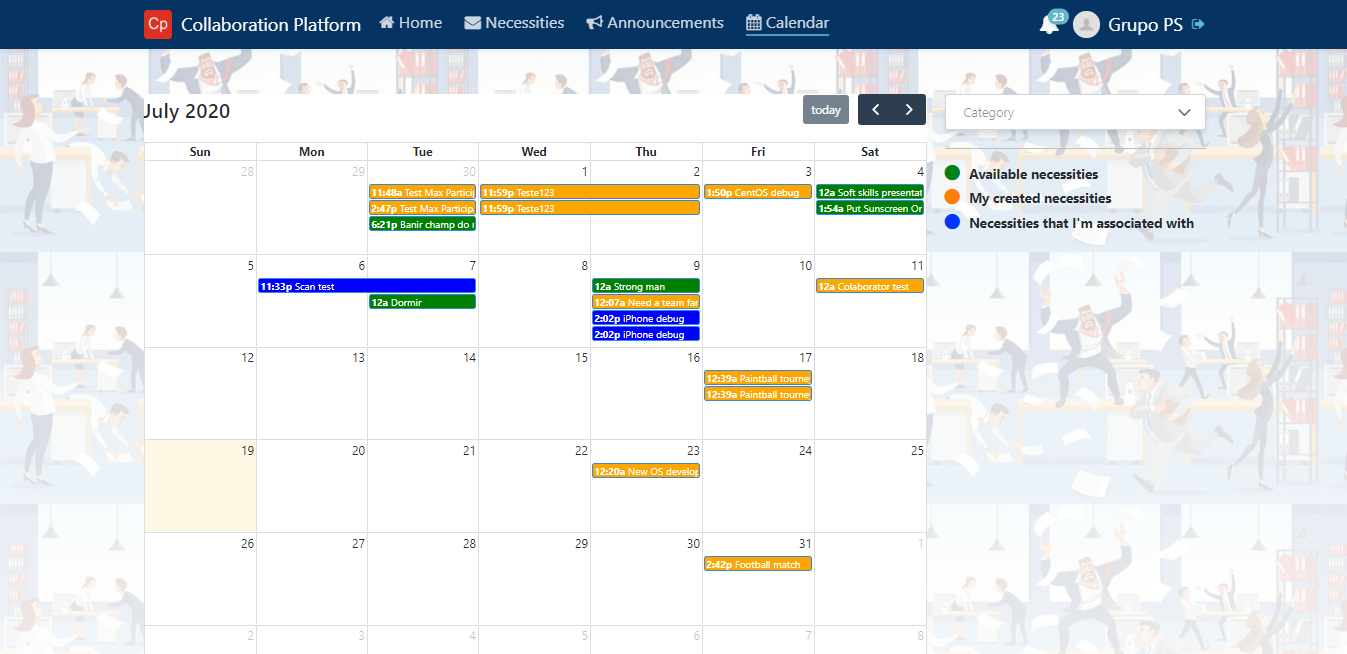
\includegraphics[scale=0.4]{figures/Calendar.png}
  \caption{Ecrã do calendário.}\label{fig:CalendarScreen}
\end{figure}

\newpage

\subsection{Criação e edição de necessidades}\label{subsec:implementacao:necessityCreation}

O ecrã \textit{NecessityCreation} (figura~\ref{fig:necessityCreation1} e~\ref{fig:necessityCreation2}) é utilizado para criar, editar, remover, arquivar ou ver os detalhes de uma necessidade.
\par
No momento da criação de uma necessidade os \textit{widgets} presentes neste ecrã permitem que o utilizador indique o título, a descrição, a categoria a qual associar a necessidade, a sua prioridade, 
se existe filtragem de participantes ou todas as candidaturas são aceites, o número máximo de participantes, uma imagem e um ficheiro para serem associados à necessidade, a data em que a mesma irá decorrer e se é necessário colaborador(es) e a data limite para a(s) sua(s) candidatura(s).

\begin{figure}[H]
  \centering 
  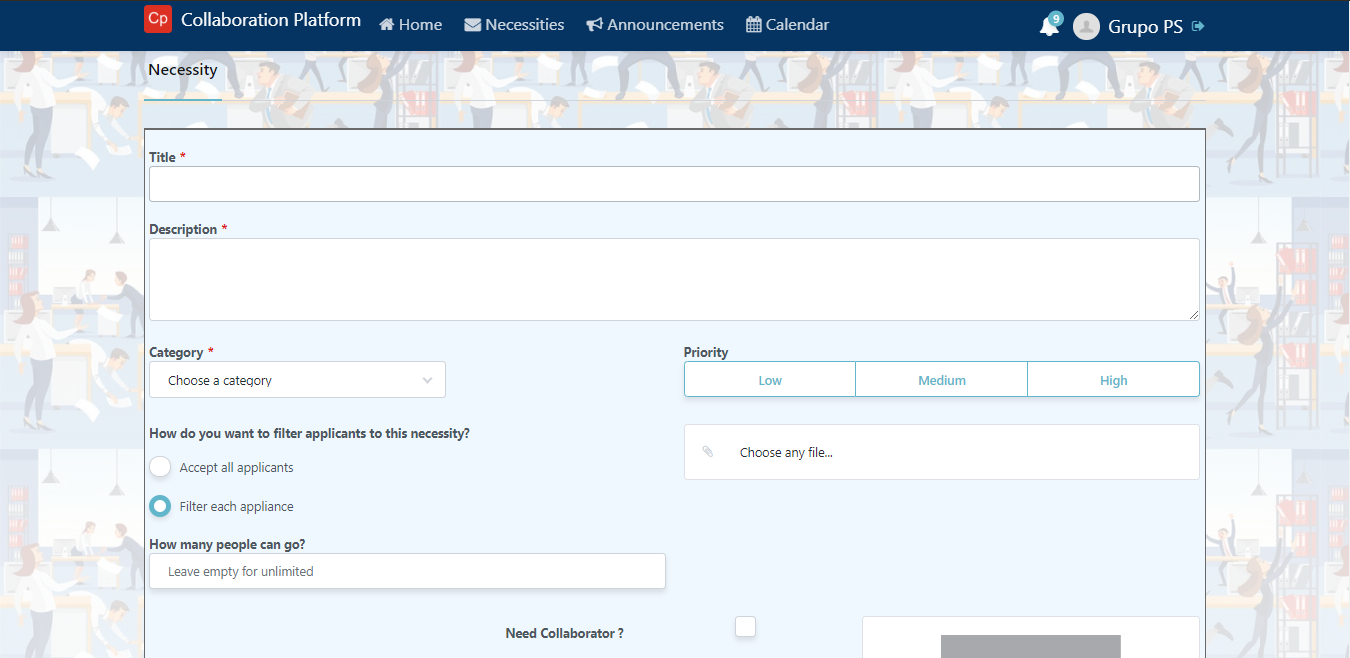
\includegraphics[scale=0.4]{figures/NecessityCreation1.png}
  \caption{Ecrã \textit{Necessity Creation} --- Criação parte 1}\label{fig:necessityCreation1}
\end{figure}



\begin{figure}[H]
  \centering 
  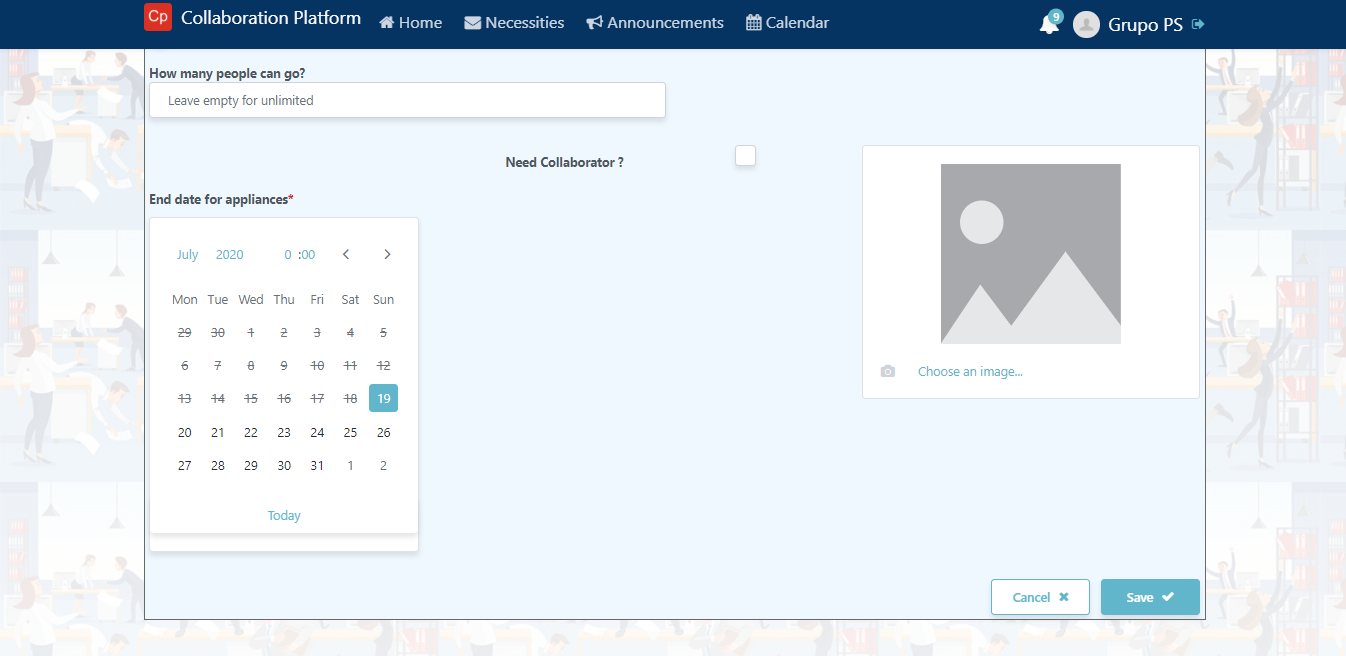
\includegraphics[scale=0.3]{figures/NecessityCreation2.png}
  \caption{Ecrã \textit{Necessity Creation} --- Criação parte 2}\label{fig:necessityCreation2}
\end{figure}


Ao pressionar o botão presente no final do ecrã com a legenda \textit{Save}, tanto num cenário de edição como de criação, 
são guardadas as informações presentes nos \textit{widgets} e é desencadeada uma \textit{client action} que posteriormente cria uma ligação ao servidor através da chamada a uma \textit{server action} para modificar a base de dados com uma nova necessidade ou alterando uma necessidade pré-existente.

Se o utilizador desejar editar ou remover uma necessidade, só o poderá fazer se for o autor desta e, no caso de a editar, após pressionar o ícone de editar o ecrã (figura~\ref{fig:NecessityCreationWithResourcesAndParticipants}) apresentará os campos já preenchidos com os dados atuais da necessidade e a possibilidade de os alterar livremente.
Um utilizador que seja um colaborador de uma dada necessidade pode também editá-la, mas não tem permissões para a eliminar.

\begin{figure}[H]
  \centering 
  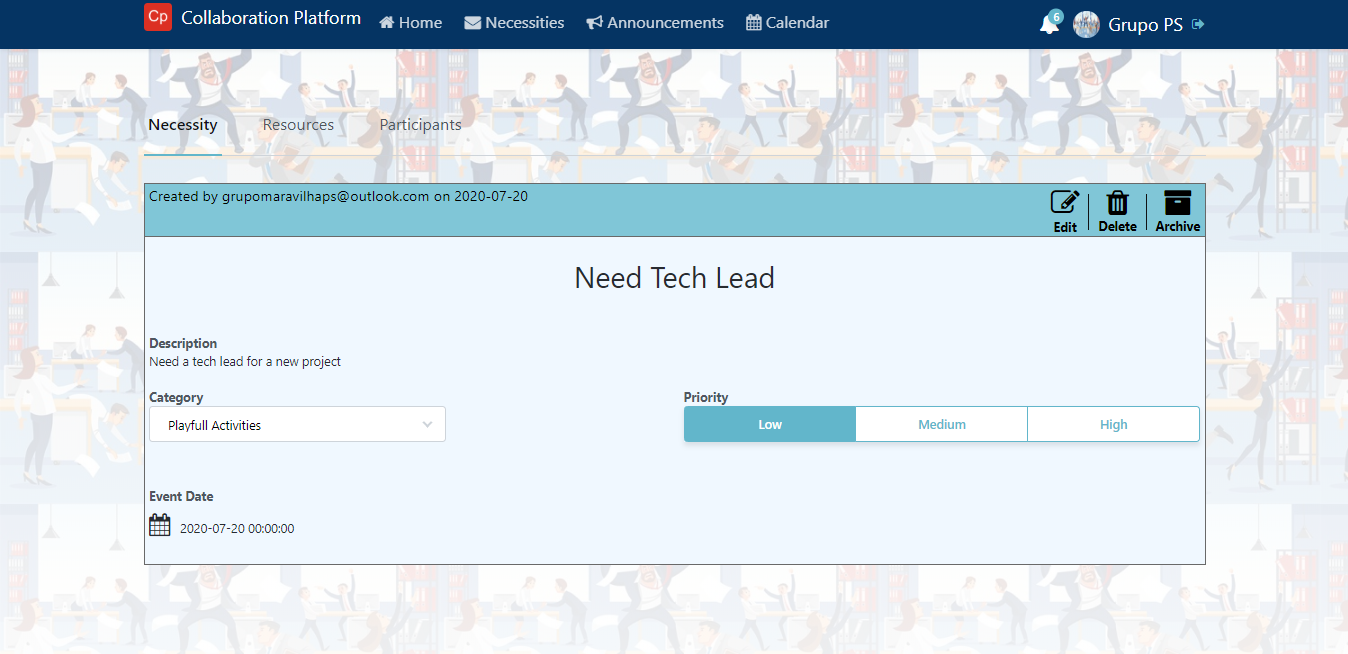
\includegraphics[scale=0.4]{figures/NecessityCreationWithResourcesAndParticipants.png}
  \caption{Ecrã \textit{Necessity Creation} --- Aba de detalhe da necessidade.}\label{fig:NecessityCreationWithResourcesAndParticipants}
\end{figure}


É também neste ecrã (figura~\ref{fig:Resources1}) que o utilizador poderá consultar os recursos associados através da navegação até à tab \textit{Resources} e, se for o autor da necessidade, pode adicionar novos recursos ou editar os existentes. 
\par
Um utilizador que seja participante numa dada necessidade pode usufruir dos recursos associados à mesma.
Para um dado recurso, o participante pode escolher usufruir deste pressionando o botão \textit{Confirm Attendance}.
\par
O autor da necessidade, assim como os colaboradores associados, podem fazer \textit{download} de um ficheiro \textit{excel} cujo conteúdo consiste nos utilizadores que vão a determinado recurso. 
Esta funcionalidade permite, de uma forma flexível, saber quem são os participantes que vão a determinado recurso.
Todos os recursos, com exceção do recurso transporte, têm um \textit{block} que contém um mapa do \textit{Google Maps} através do qual o utilizador pode colocar um marker para dar a conhecer a localização associada ao recurso. 
\par
A integração do \textit{Google Maps} (figura~\ref{fig:Resources2}) na plataforma é realizada através da comunicação com a API do \textit{Google Maps}~\cite{google maps api}. 
Para criar um novo mapa é necessário criar um objeto do tipo \textit{google.maps.Map} que recebe na sua construção o elemento \textit{html} onde o mapa será inserido. 
Toda a dinâmica de interação com o mapa é gerida pela API através de eventos que são desencadeados com o toque no mesmo. 
Para efeitos de reduzir a quantidade de pedidos feitos à API \textit{Google Maps JavaScript API} com o incentivo de obter um mapa, cada mapa é guardado num objeto \textit{maps} que funciona como um contentor de objetos de mapas e os seus marcadores.
Cada mapa é inicializado apenas quando for necessário mostrá-lo em conjunto com um recurso da necessidade, como visto na figura~\ref{fig:googleMapsInitCode}.

\begin{figure}[H]
  \centering 
  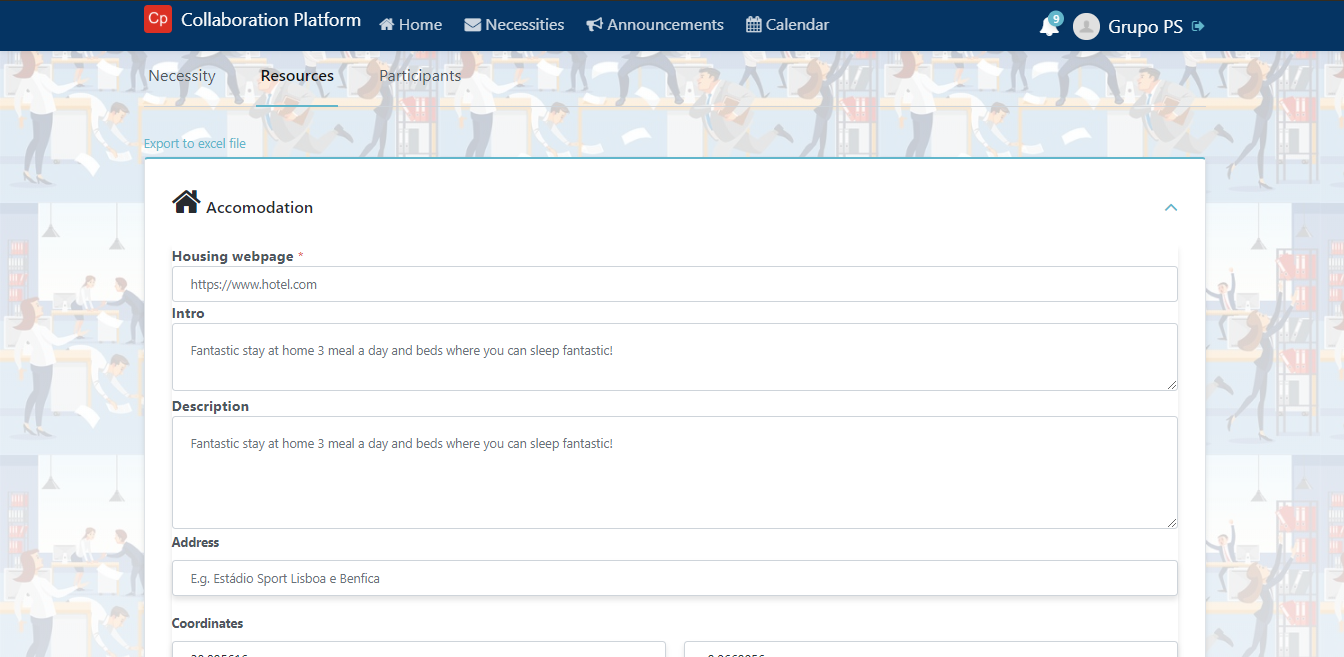
\includegraphics[scale=0.4]{figures/Resources1.png}
  \caption{Ecrã \textit{Necessity Creation} --- Aba de recursos parte 1.}\label{fig:Resources1}
\end{figure}



\begin{figure}[H]
  \centering 
  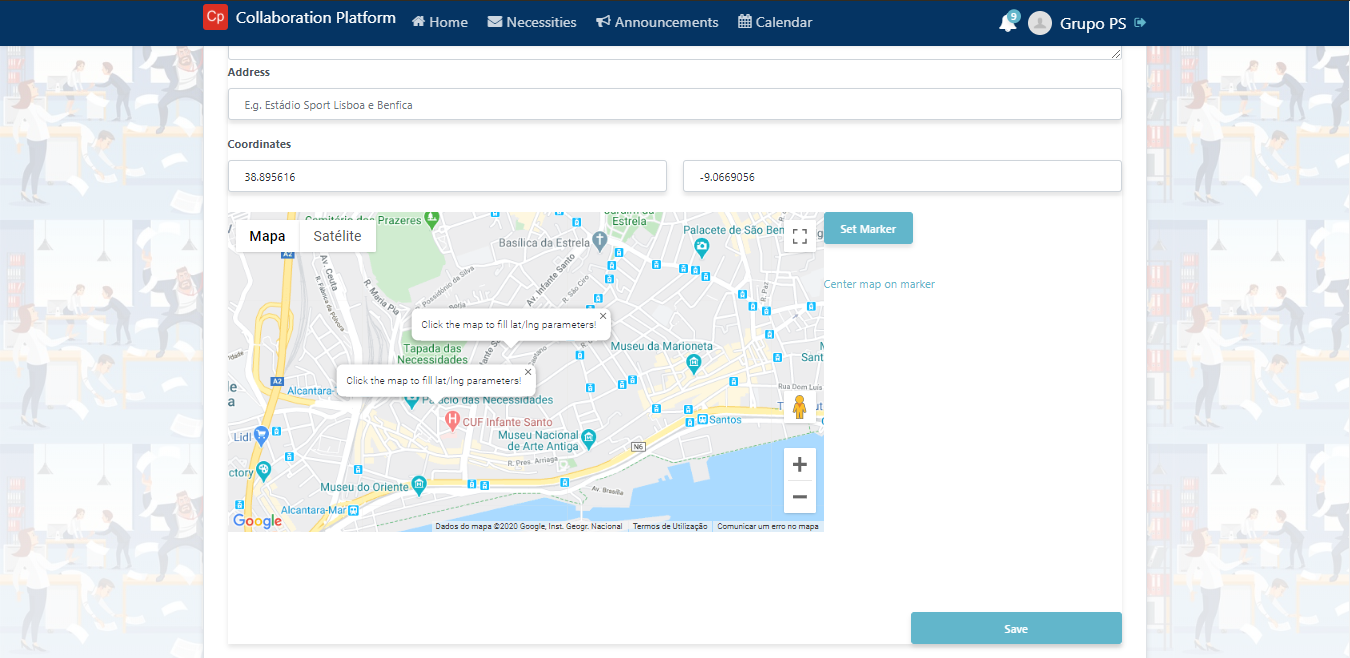
\includegraphics[scale=0.4]{figures/Resources2.png}
  \caption{Ecrã \textit{Necessity Creation} --- Aba de recursos parte 2.}\label{fig:Resources2}
\end{figure}


\begin{figure}[H]
  \centering 
  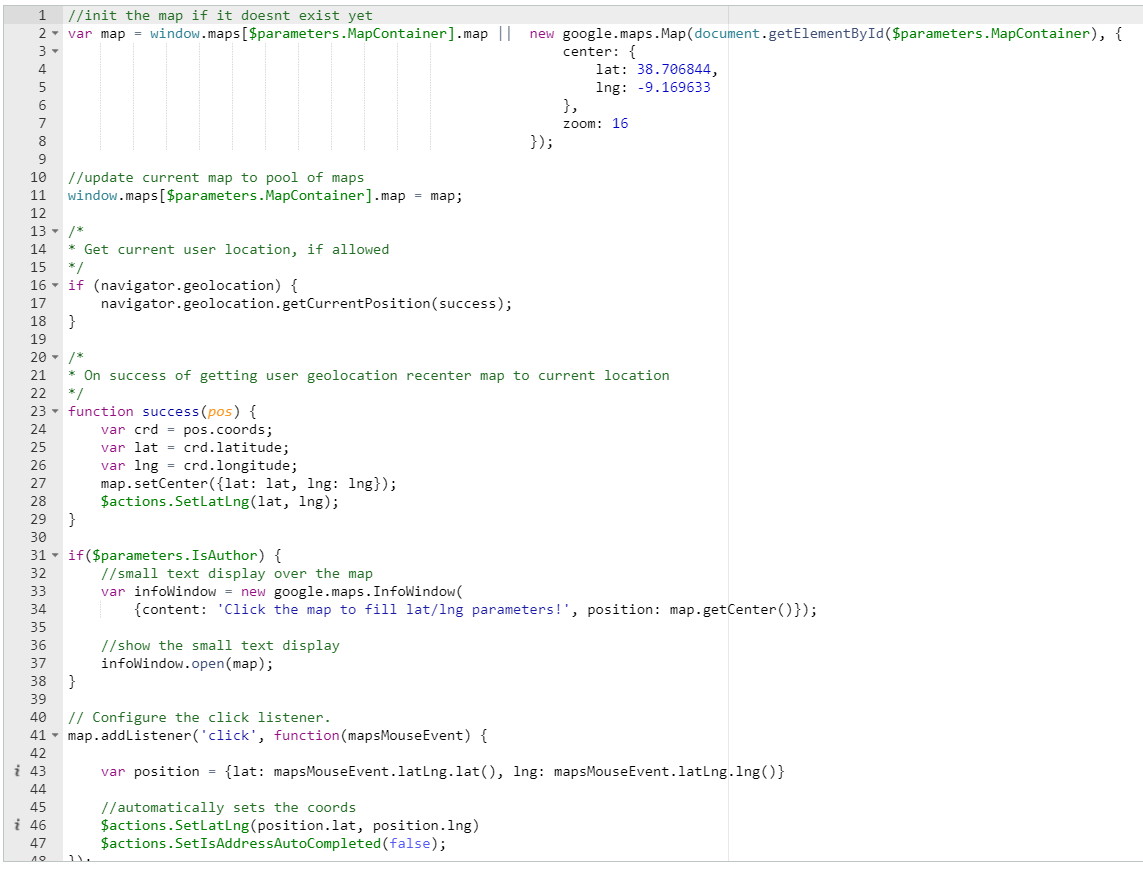
\includegraphics[scale=0.4]{figures/googleMapsInitCode.png}
  \caption{Listagem de código para inicialização do \textit{Google Maps}}\label{fig:googleMapsInitCode}
\end{figure}


Na última tab do \textit{widget Tabs} presente no ecrã \textit{NecessityCreation} (figura~\ref{fig:participants}) encontra-se a secção relacionada com os participantes à necessidade.
Toda a dinâmica relativa a esta tab \textit{"Participants"} do ecrã \textit{NecessityCreation} é suportada por um \textit{Web Block} denominado \textit{ParticipantsBlock}.
Nesta secção um utilizador poderá candidatar-se à posição de colaborador ou participante, de acordo com a fase em que a necessidade se encontra, carregando no \textit{widget link} com o texto \textit{Apply as a Colaborator/Participant} e deixando uma descrição, se a filtragem dos candidatos estiver ativa para aquela necessidade.
\par
Um utilizador, ao criar uma necessidade, tem a opção de escolher se todas as candidaturas são aceites ou se o próprio irá proceder à sua filtragem selecionando um dos \textit{widgets radio button}.  

\begin{figure}[H]
  \centering 
  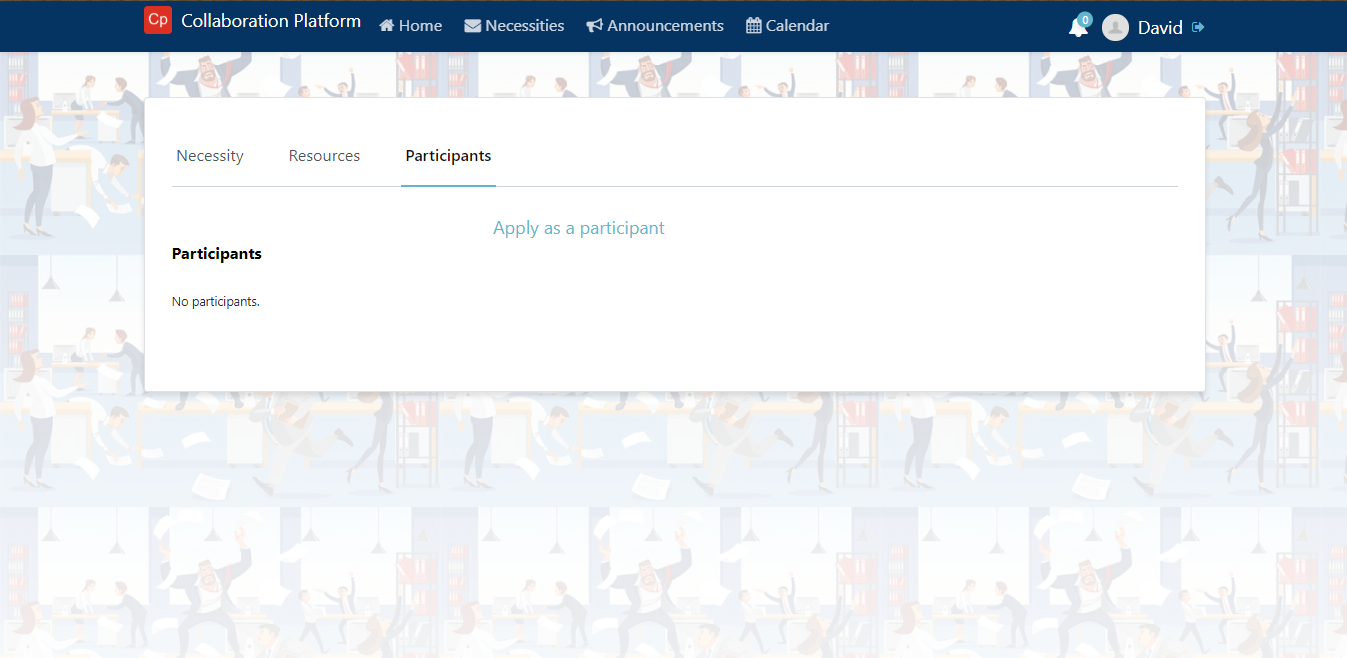
\includegraphics[scale=0.4]{figures/Participants.png}
  \caption{Ecrã \textit{Necessity Creation} --- Aba dos participantes - Candidatura.}\label{fig:participants}
\end{figure}

Considere-se que um participante quer remover a sua participação a uma dada necessidade; no caso de ainda não ter sido aceite, isto é, a sua candidatura à necessidade está pendente, o cancelamento é instantâneo ao pressionar o botão \textit{Cancel participation} (apresentado no ecrã da (figura~\ref{fig:participants_removal})).
Se já tiver sido aceite, ao carregar no botão \textit{Cancel participation} irá ser enviada uma notificação para o autor e para os colaboradores da necessidade para que removam este participante da lista. 
O utilizador, ao pressionar este botão, é desencadeada uma \textit{client action} que posteriormente comunica com o servidor através de uma \textit{server action} para que este participante seja marcado para remover na base de dados.

\begin{figure}[H]
  \centering 
  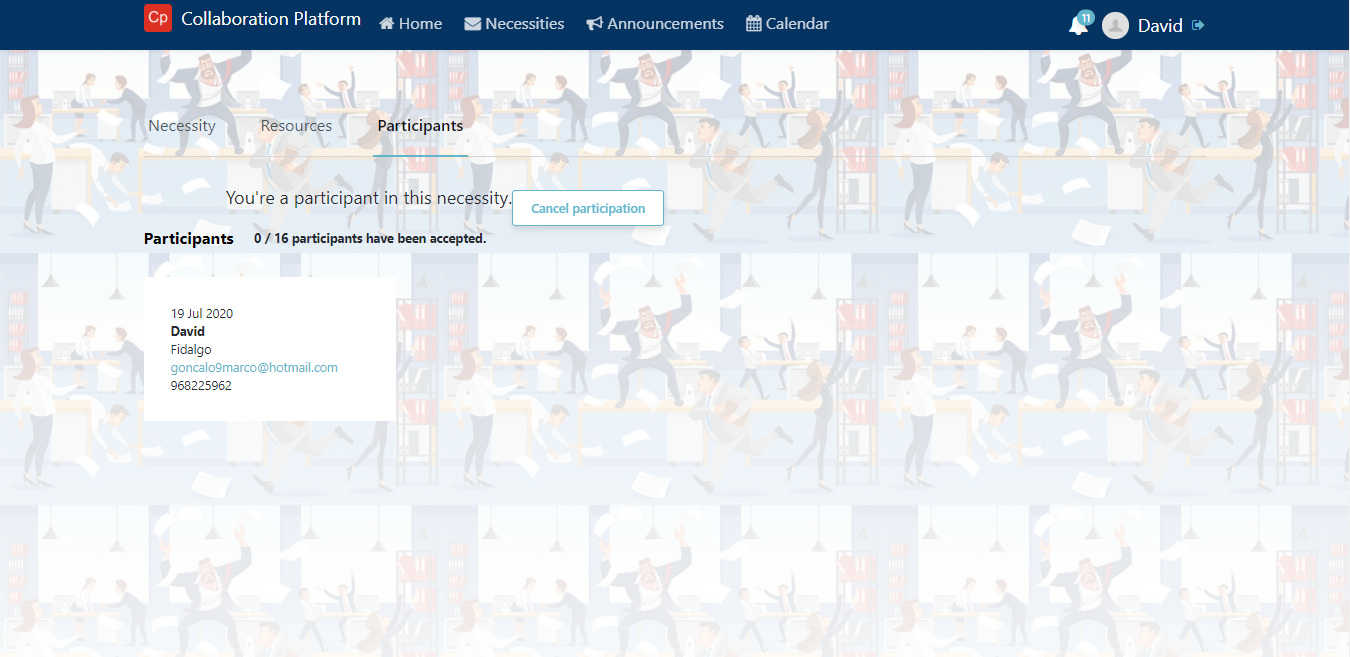
\includegraphics[scale=0.4]{figures/Participants_removal.png}
  \caption{Ecrã \textit{Necessity Creation} --- Aba dos participantes - Candidatura efetuada.}\label{fig:participants_removal}
\end{figure}


Na lista dos participantes de uma necessidade (apresentada no ecrã da (figura~\ref{fig:participants_removal2})), um utilizador que esteja marcado para remover apresenta um ícone a vermelho onde um utilizador que seja o autor ou colaborador pode carregar para o remover. 
Apenas utilizadores que tenham pedido para cancelar a sua participação podem ser removidos.

\begin{figure}[H]
  \centering 
  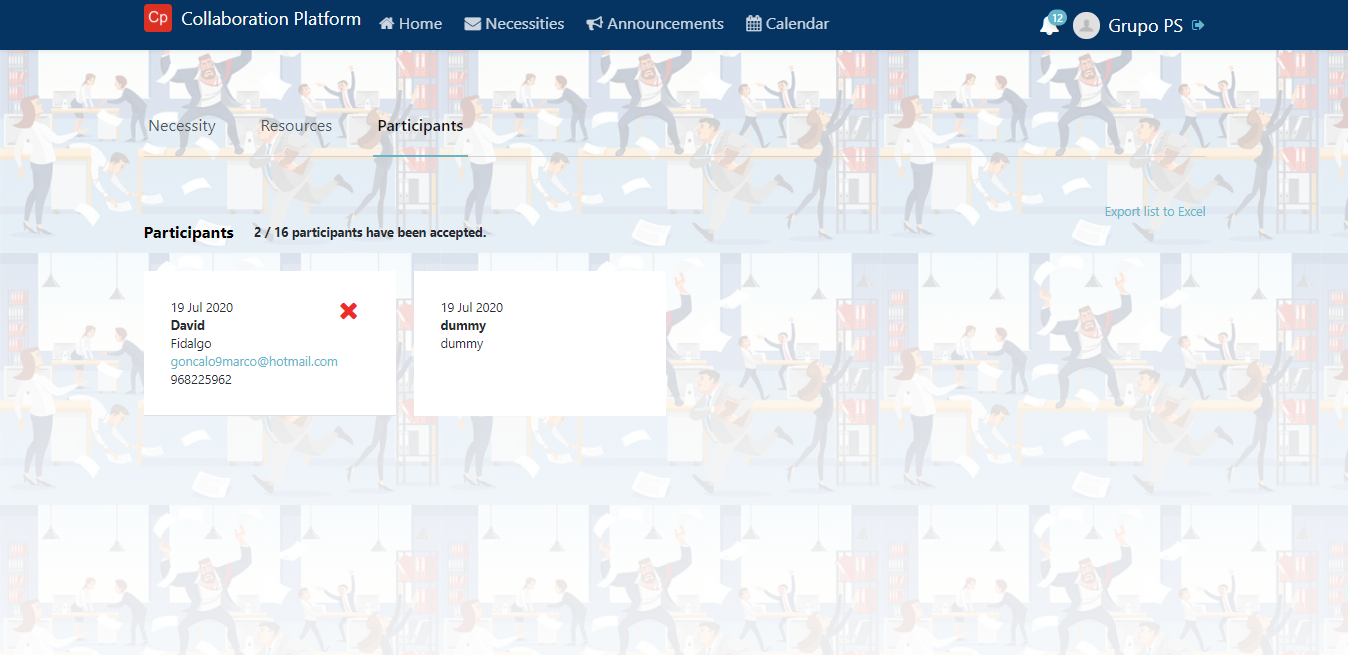
\includegraphics[scale=0.4]{figures/Participants_removal2.png}
  \caption{Ecrã \textit{Necessity Creation} --- Aba dos participantes - Remoção de um participante da lista.}\label{fig:participants_removal2}
\end{figure}


\newpage


\subsection{Geração e leitura de \textit{QR Code} para marcação de presença}\label{subsec:implementacao:qrcode}

A geração de \textit{QR code}, para a confirmação de presença numa necessidade caso a categoria da mesma suporte QR code,
 é feita pelo \textit{timer VerifyNecessityDateToGenerateQRCode} (ver subsecção~\ref{subsec:implementacao:timers}) no dia de evento definido pelo autor. 
\par
 Para cada participante será gerado um QR code único para ser lido por um colaborador ou o próprio autor da necessidade em questão.
\par
Semelhante à metodologia de geração de QR codes, é disponibilizado um ecrã de leitura de QR codes apenas visível a colaboradores e autores das respectivas necessidades, estes são notificados da disponibilização do ecrã.
Neste ecrã irá ser pedido ao utilizador permissões de utilização da câmara, como visto na figura~\ref{fig:cameraCode}, para realizar uma leitura contínua de QR codes pressionando no botão \textit{Scan QR Codes} e de seguida no \textit{Capture} para capturar o conteúdo visto na câmara, se existir um QR code irá ser apresentado uma mensagem de sucesso caso contrário uma mensagem de erro a avisar o utilizador que não foi possível encontrar nenhum QR code.
Para realizar o acesso à câmera foi necessário entender os conceitos de \textit{constraints} que é um objeto de \textit{MediaStreamConstraints} que contém informações sobre o tipo de \textit{media} no pedido e os requisitos de cada pedido~\cite{mediastreamconstraints}.

\begin{figure}[H]
  \centering 
  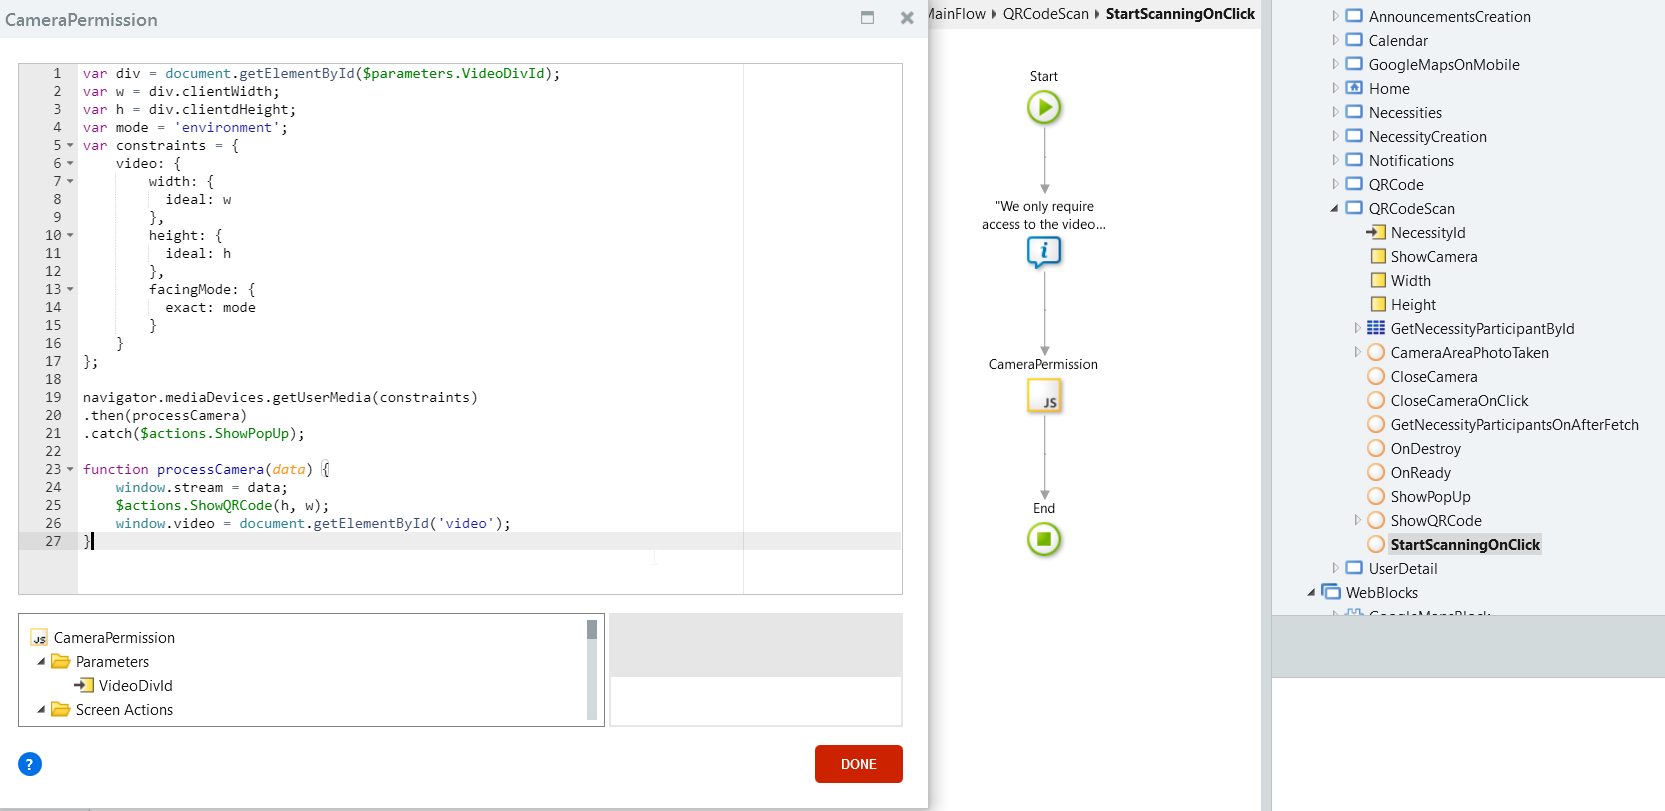
\includegraphics[scale=0.4]{figures/CameraCode.png}
  \caption{Listagem de código para acesso à câmera.}\label{fig:cameraCode}
\end{figure}

\newpage


\subsection{Edição de perfil do utilizador}\label{subsec:implementacao:editprofile}

Com o objetivo de editar o seu perfil, um utilizador ao carregar no seu nome navega até ao ecrã \textit{UserDetail}, representado na figura~\ref{fig:user_detail}. 
\par
No contexto deste ecrã, um utilizador tem oportunidade de alterar os campos associados ao seu perfil, nomeadamente o seu nome, nome de utilizador, email, número de telefone e a imagem de perfil.
\par 
É importante referir que o \textit{upload} de imagens ou ficheiros de tamanho considerável faz com que a comunicação com o servidor se torne lenta e, em casos extremos, a mesma pode resultar numa exceção do tipo \textit{\" connection timed out\".}
 
\begin{figure}[H]
  \centering 
  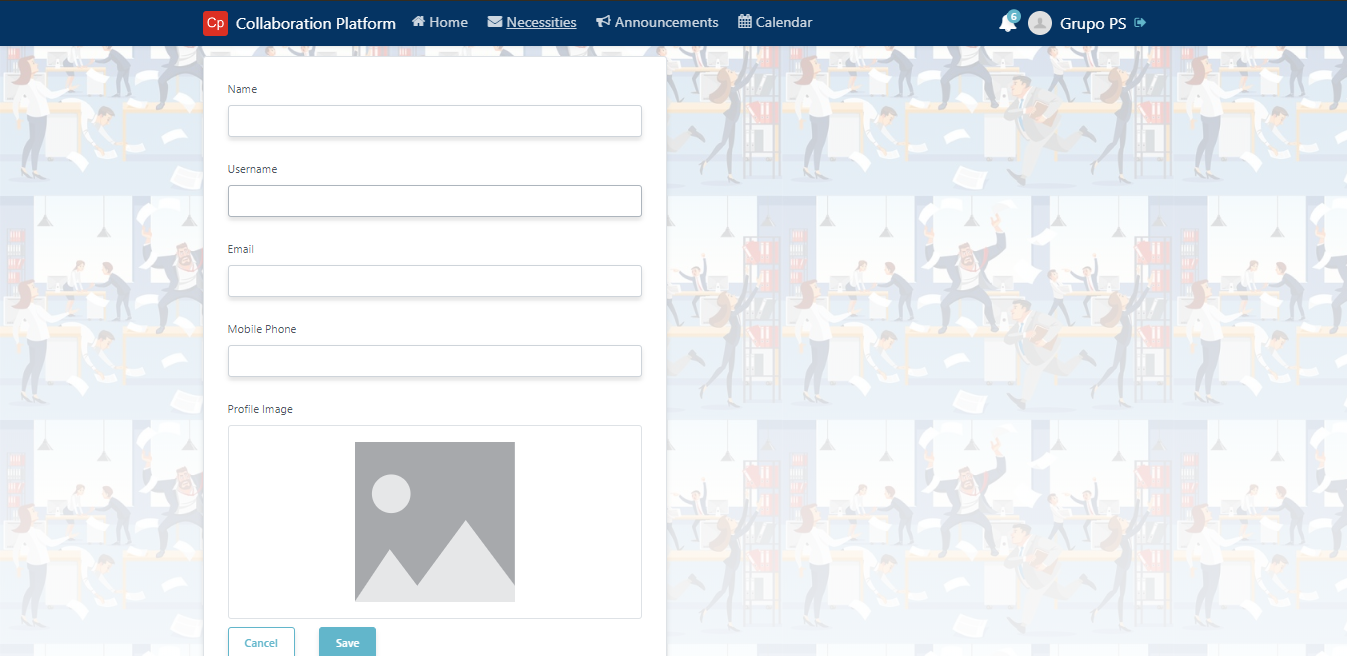
\includegraphics[scale=0.4]{figures/user_detail.png}
  \caption{Ecrã \textit{UserDetail} }\label{fig:user_detail}
\end{figure}



\subsection{Notificações na plataforma}\label{subsec:implementacao:notificacoes}

A plataforma tem um sistema de notificações que suporta o seu envio para os utilizadores, num ecrã (figura~\ref{fig:notifications}) onde é possível visualizá-las em detalhe. 
\par
Os cenários possíveis de envio de notificações consistem em: 
sempre que existir uma nova candidatura a uma dada necessidade o autor da mesma é notificado; 
quando um utilizador vê a sua candidatura aceite ou não; 
quando uma necessidade é eliminada ou editada, os participantes da mesma são notificados;
quando um dado utilizador quer desistir da sua participação a uma necessidade, o autor da mesma recebe uma notificação para remover esse participante;
quando uma mensagem enviada para os administradores da plataforma foi resolvida ou rejeitada;
e, por último, quando é o dia em que uma necessidade se vai realizar e a mesma tem \textit{QR code} associado, os participantes recebem uma notificação com um link para o \textit{QR code} gerado.
\par
A cada notificação está associado o \textit{id} do utilizador, o que permite que quando o mesmo navegue até ao ecrã das notificações, 
lhe sejam apresentadas todas as suas notificações que recebeu, provenientes do registo na base de dados.

\begin{figure}[H]
  \centering 
  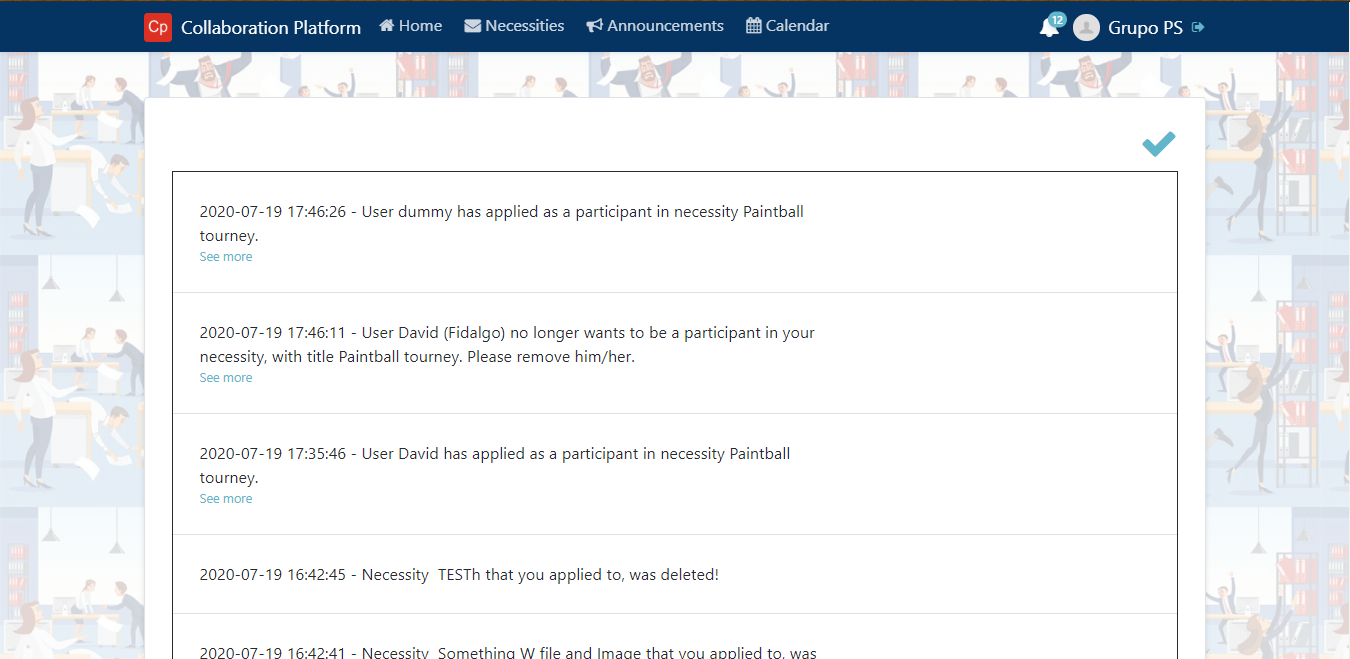
\includegraphics[scale=0.4]{figures/Notifications.png}
  \caption{Ecrã \textit{Notifications}}\label{fig:notifications}
\end{figure}

\newpage

\subsection{Comunicados na plataforma}\label{subsec:implementacao:comunicados}

A divulgação de comunicados na \textit{Collaboration Platform} tem como objetivo a transmissão de informação de forma uniforme por todos os utilizadores registados.
\par
Um utilizador autenticado acede ao ecrã \textit{Announcements} (figura~\ref{fig:announcements}) e verifica os comunicados, apresentados sob a forma de uma lista. 
A seleção de um destes comunicados apresenta os detalhes do mesmo, visto que cada comunicado é apresentado num \textit{widget Accordion}. 
Um utilizador com permissões de administrador ou o \textit{owner}, ao navegar para o ecrã \textit{Announcements}, têm a possibilidade de criar um novo comunicado pressionando o botão \textit{Create Announcement}, criação esta que é completada no ecrã \textit{AnnouncementsCreation} (figura~\ref{fig:announcement_creation}).
\par
Cada comunicado tem associado um título, uma descrição e, facultativamente, um ficheiro e uma imagem.

\begin{figure}[H]
  \centering 
  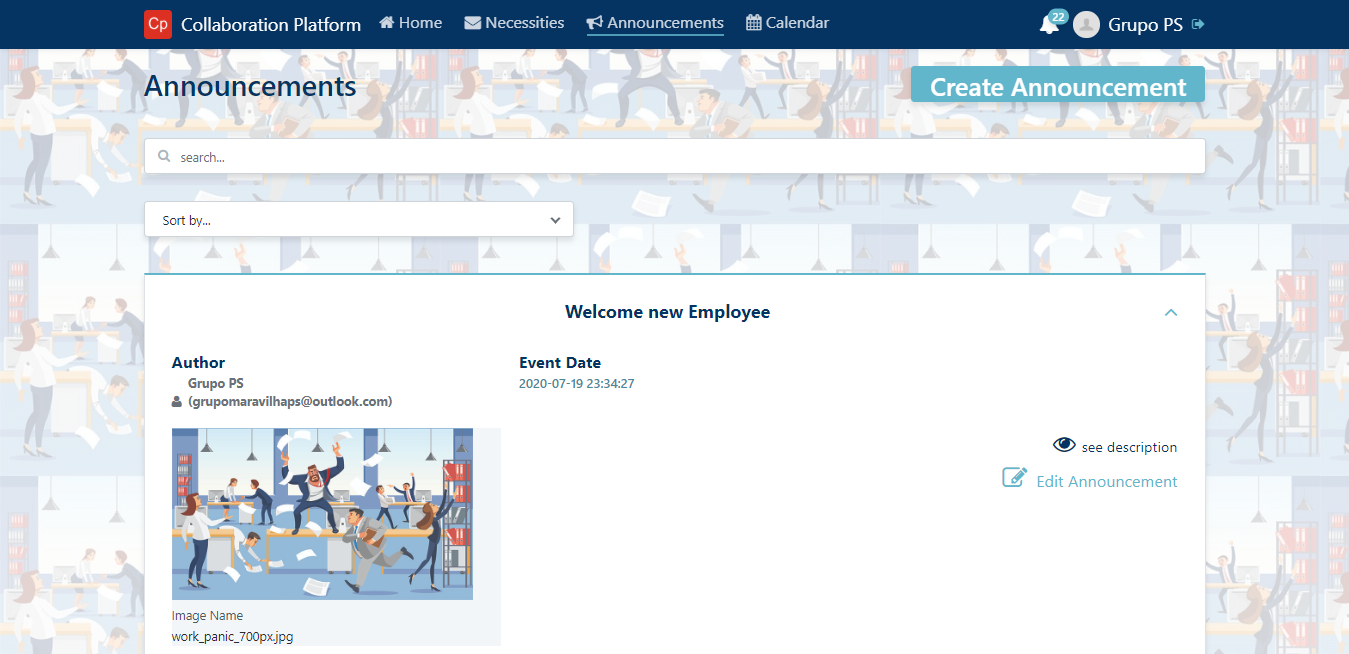
\includegraphics[scale=0.4]{figures/Announcements.png}
  \caption{Ecrã \textit{Announcements}}\label{fig:announcements}
\end{figure}



\begin{figure}[H]
  \centering 
  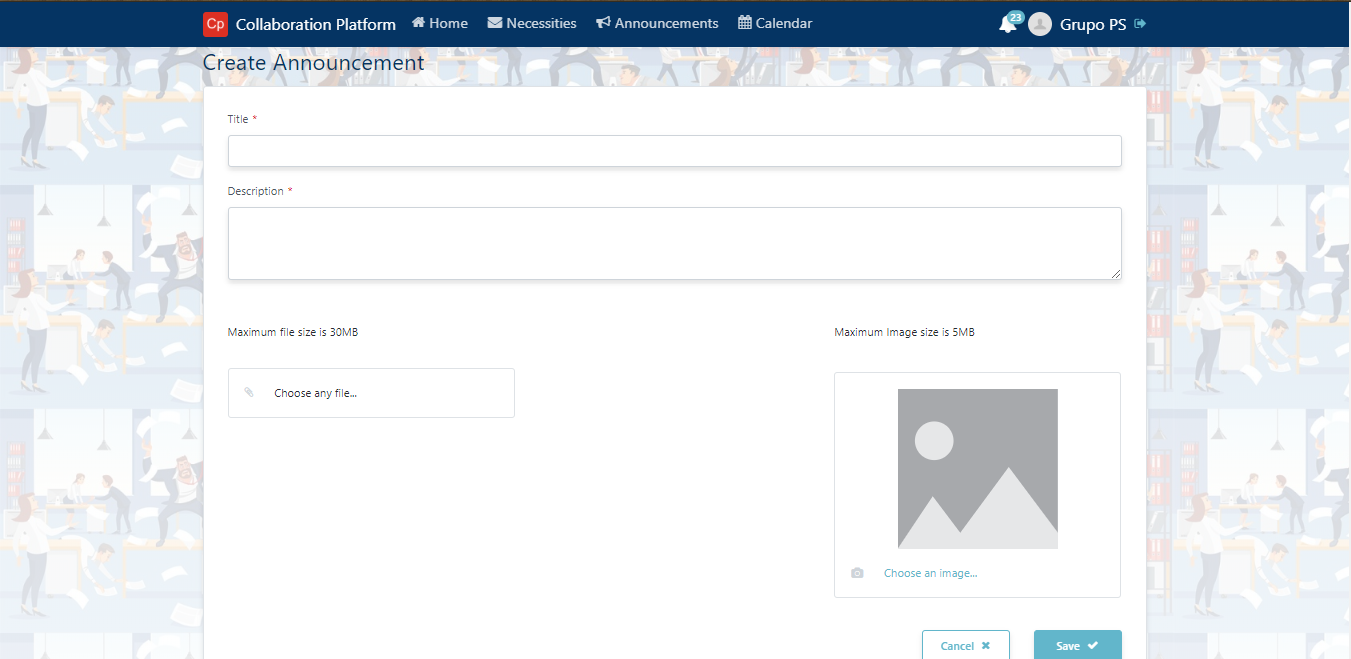
\includegraphics[scale=0.4]{figures/AnnouncementCreation.png}
  \caption{Ecrã \textit{AnnouncementCreation}}\label{fig:announcement_creation}
\end{figure}

\newpage

\subsection{Implementação de \textit{timers}}\label{subsec:implementacao:timers}

A plataforma \textit{OutSystems~\cite{outsystems}} oferece um serviço, representado na figura~\ref{fig:timers}, que permite executar lógica de forma assíncrona, isto é, executa uma dada ação (\textit{task}) de forma periódica. 

\begin{figure}[H]
  \centering 
  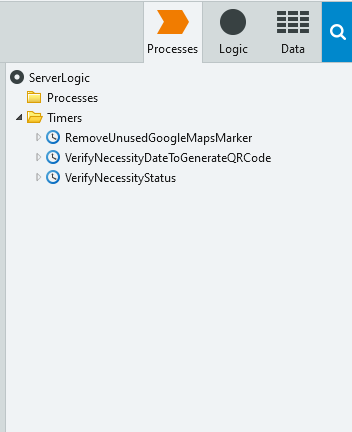
\includegraphics[scale=0.4]{figures/timers.png}
  \caption{Timers implementados}\label{fig:timers}
\end{figure}

Deste modo, no contexto da \textit{Collaboration Platform} foram desenvolvidos três \textit{timers} com propósitos distintos, apresentados na figura~\ref{fig:timers}.

\par
O \textit{timer RemoveUnusedGoogleMapMarker}, representado na figura~\ref{fig:timer1}, corre semanalmente com o propósito de remover todos os marcadores do \textit{Google Maps} (textit{markers}) que tenham o contador de utilização a 0. 
\par 
Este \textit{timer} é necessário devido ao facto dos \textit{markers} serem partilhados entre necessidades, ou seja, necessidades com 
 a mesma localização partilham o mesmo marcador. Esta otimização permite poupar espaço na base de dados.

 \begin{figure}[H]
  \centering 
  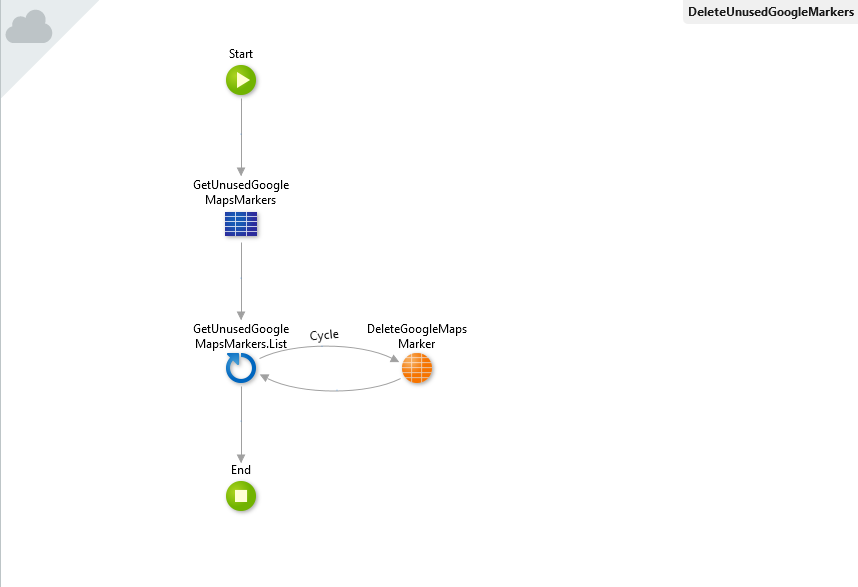
\includegraphics[scale=0.4]{figures/timer1.png}
  \caption{\textit{Timer RemoveUnusedGoogleMapMarker}}\label{fig:timer1}
\end{figure}


\par
O \textit{timer VerifyNecessityDateToGenerateQRCode}, representado na figura~\ref{fig:timer2}, corre diariamente para encontrar as necessidades que irão decorrer no presente dia e que necessitem de QR Code para verificação de presença dos participantes. 
Quando encontra, procede à geração do QR Code e envia notificações aos participantes da necessidade para que os mesmo o possam apresentar.

\begin{figure}[H]
  \centering 
  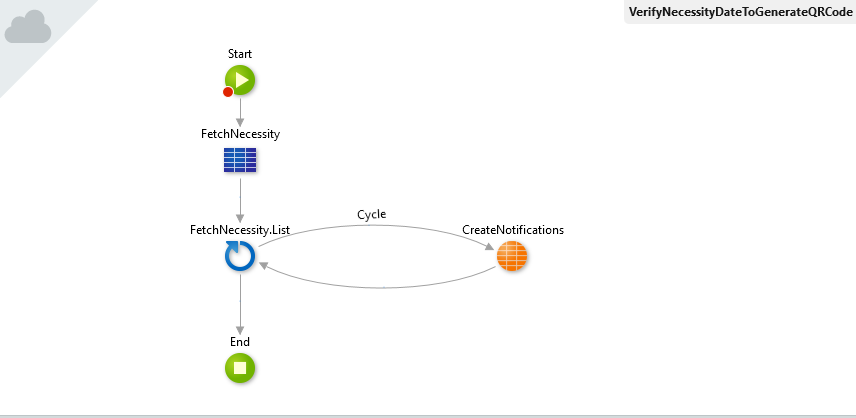
\includegraphics[scale=0.4]{figures/timer2.png}
  \caption{\textit{Timer VerifyNecessityDateToGenerateQRCode}}\label{fig:timer2}
\end{figure}


\par
O \textit{timer VerifyNecessityStatus}, representado na figura~\ref{fig:timer3}, corre diariamente para encontrar as necessidades que tenham ocorrido no dia anterior e é imperativo mudar o seu estado de \textit{active} para \textit{closed}. 

\begin{figure}[H]
  \centering 
  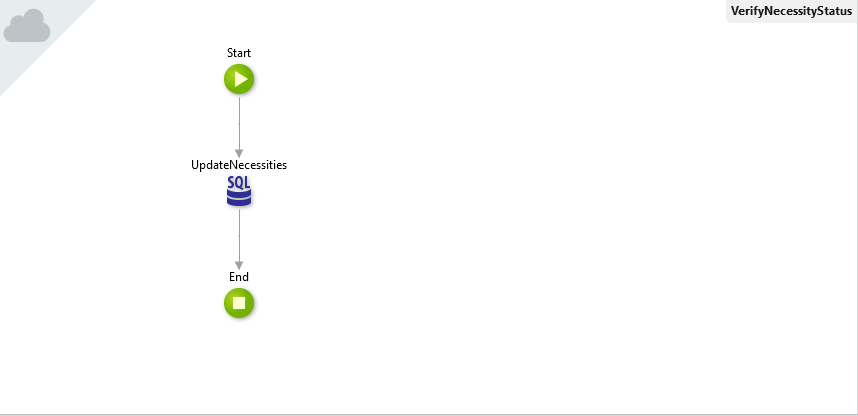
\includegraphics[scale=0.4]{figures/timer3.png}
  \caption{\textit{Timer VerifyNecessityStatus}}\label{fig:timer3}
\end{figure}
